\documentclass[aspectratio=169, t, 9pt]{beamer} % 16:9 ratio, t: top alignment, 9pt: default text size

%%%%%%%%%%%%%%%%%%%%%%%%%%%%%%%%%%%%%%%%%%%%%%%%%%%%%%%%%%%%%%%%%%%%%%%%%%%%%%%%
% Titlepage information
\title[CMOS+X] %optional
{}

% \subtitle{Status report and feedback}
\subtitle{Cryo-CMOS power management}

\author[] % (optional, for multiple authors)
% {A.~Alpha\inst{1} \and B.~Bravo\inst{2} \\ On behalf of Institute X, Institute Y, Institute Z}
{Llorenç Fanals-i-Batllori\inst{1,\textdagger} \\ \inst{1}SLAC National Accelerator Laboratory \\ \inst{\textdagger}\href{mailto:fanals@slac.stanford.edu}{fanals@slac.stanford.edu}}

\institute[SLAC] % (optional)
{
  \inst{1}%
  Faculty of Foo\\
  Bar University
  \and
  \inst{2}%
  Faculty of Baz\\
  Quz University
}

% \date{\today}% (optional)
\date{2026/10/20}% (optional)
%%%%%%%%%%%%%%%%%%%%%%%%%%%%%%%%%%%%%%%%%%%%%%%%%%%%%%%%%%%%%%%%%%%%%%%%%%%%%%%%

\usepackage[default]{lato} % set Lato as the default font
\usepackage{svg} % includesvg{foo.svg}
\usepackage{tikz} % graphics
\usepackage{circuitikz} % circuits
\usetikzlibrary{decorations.pathreplacing} % brackets
\usetikzlibrary{arrows.meta,shapes} % signal arrow
\usepackage{makecell}
\usetikzlibrary{arrows}
\usepackage{siunitx} % SI units
\sisetup{per-mode=fraction}
\DeclareSIUnit{\square}{\ensuremath{\square}}
\usepackage{graphicx,transparent} % graphics
\usepackage{pgfplots} % tikz plots
\usepgfplotslibrary{colorbrewer} % cycle color
\usepackage{filecontents} % read csvs
% \usepackage[natbib=true,backend=bibtex,sorting=none]{biblatex}
% \bibliography{./bibliography.bib}
\usepackage[style=numeric, backend=biber, maxcitenames=1, mincitenames=1]{biblatex}
\renewbibmacro*{name:andothers}{}
\addbibresource{./bibliography.bib}
  \DeclareCiteCommand{\cite}[\mkbibbrackets]
    {\usebibmacro{prenote}}
    {\usebibmacro{citeindex}%
     \printfield{labelnumber}%
     \setunit{\addcomma\space}%
     \printnames[family][1-1]{labelname}%
     \setunit{\addspace}%
     \printfield{year}}
    {\multicitedelim}
    {\usebibmacro{postnote}}



\usepackage{hyperref} % mailto
\usepackage{listings}
\usepackage[para]{threeparttable}

\lstset{
    basicstyle=\ttfamily\small,
    frame=single,
    backgroundcolor=\color{gray!10},
}


% Import template
% Import palette
% Color palette, https://identity.stanford.edu/design-elements/color/primary-colors/
% Primary
\definecolor{cardinal}{HTML}{8C1515}
\definecolor{cardinal_light}{HTML}{B83A4B}
\definecolor{cardinal_dark}{HTML}{820000}
\definecolor{stanford_white}{HTML}{FFFFFF}
\definecolor{stanford_black}{HTML}{2E2D29}
\definecolor{cool_grey}{HTML}{53565A}
% Accent colors
\definecolor{paloalto}{HTML}{175E54}
\definecolor{paloalto_light}{HTML}{2D716F}
\definecolor{paloalto_dark}{HTML}{014240}
\definecolor{paloverde}{HTML}{279989}
\definecolor{paloverde_light}{HTML}{59B3A9}
\definecolor{paloverde_dark}{HTML}{017E7C}
\definecolor{olive}{HTML}{8F993E}
\definecolor{olive_light}{HTML}{A6B168}
\definecolor{olive_dark}{HTML}{7A863B}
\definecolor{bay}{HTML}{6FA287}
\definecolor{bay_light}{HTML}{8AB8A7}
\definecolor{bay_dark}{HTML}{417865}
\definecolor{sky}{HTML}{4298B5}
\definecolor{sky_light}{HTML}{67AFD2}
\definecolor{sky_dark}{HTML}{016895}
\definecolor{lagunita}{HTML}{007C92}
\definecolor{lagunita_light}{HTML}{009AB4}
\definecolor{lagunita_dark}{HTML}{006B81}
\definecolor{poppy}{HTML}{E98300}
\definecolor{poppy_light}{HTML}{F9A44A}
\definecolor{poppy_dark}{HTML}{D1660F}
\definecolor{spirited}{HTML}{E04F39}
\definecolor{spirited_light}{HTML}{F4795B}
\definecolor{spirited_dark}{HTML}{C74632}
\definecolor{illuminating}{HTML}{FEDD5C}
\definecolor{illuminating_light}{HTML}{FFE781}
\definecolor{illuminating_dark}{HTML}{FEC51D}
\definecolor{plum}{HTML}{620059}
\definecolor{plum_light}{HTML}{734675}
\definecolor{plum_dark}{HTML}{350D36}
\definecolor{brick}{HTML}{651C32}
\definecolor{brick_light}{HTML}{7F2D48}
\definecolor{brick_dark}{HTML}{42081B}
\definecolor{archway}{HTML}{5D4B3C}
\definecolor{archway_light}{HTML}{766253}
\definecolor{archway_dark}{HTML}{2F2424}
\definecolor{stone}{HTML}{7F7776}
\definecolor{stone_light}{HTML}{D4D1D1}
\definecolor{stone_dark}{HTML}{544948}
\definecolor{fog}{HTML}{DAD7CB}
\definecolor{fog_light}{HTML}{F4F4F4}
\definecolor{fog_dark}{HTML}{B6B1A9}
% Web interactive colors
\definecolor{digitalred}{HTML}{B1040E}
\definecolor{digitalred_light}{HTML}{E50808}
\definecolor{digitalred_dark}{HTML}{820000}
\definecolor{digitalblue}{HTML}{006CB8}
\definecolor{digitalblue_light}{HTML}{6FC3FF}
\definecolor{digitalblue_dark}{HTML}{00548F}
\definecolor{digitalgreen}{HTML}{008566}
\definecolor{digitalgreen_light}{HTML}{1AECBA}
\definecolor{digitalgreen_dark}{HTML}{006F54}


% To adjust spacings
% \usepackage{etoolbox}

% Default line spacing
\linespread{1.5}

% Apply colors
\setbeamercolor{title}{fg=cardinal}
\setbeamercolor{frametitle}{fg=cardinal}
\setbeamercolor{section in toc}{fg=cardinal}
\setbeamercolor{section title}{fg=cardinal}
\setbeamercolor{subtitle}{fg=cardinal}
\setbeamercolor{bibliography item}{fg=cardinal_dark}
\setbeamercolor{bibliography entry author}{fg=cardinal_dark}
\setbeamercolor{bibliography entry title}{fg=cardinal_light}
\setbeamercolor{bibliography entry location}{fg=cardinal}
\setbeamercolor{bibliography entry note}{fg=paloalto}

% Itemize and enumerate
\newcommand{\cardinalbullet}{\raisebox{0.5pt}{\color{cardinal}\footnotesize\textbullet}}
\setbeamertemplate{itemize item}{\cardinalbullet}
\setbeamertemplate{itemize subitem}{\cardinalbullet}
\setbeamertemplate{itemize subsubitem}{\cardinalbullet}
\setbeamertemplate{enumerate items}[default]
\setbeamercolor{enumerate item}{fg=cardinal}
\setbeamercolor{enumerate subitem}{fg=cardinal}

% \setbeamertemplate{enumerate item}{\cardinalbullet}
% \setbeamertemplate{enumerate subitem}{\cardinalbullet}
% \setbeamertemplate{enumerate subsubitem}{\cardinalbullet}


% Subtitle macro
\newcommand{\subheading}[1]{{\color{cardinal_light} \Large #1}}

% Columns environment to respect margins
\newenvironment{groupcolumns}[1][]{%
    \begin{columns}[onlytextwidth,T,#1]% 'onlytextwidth': only use available space, respect margins; 'T': align columns tops to top
}{%
    \end{columns}%
}

% Footer; on frame, use 'plain' to hide frame number and 'noframenumbering' to skip frame_counter++
\beamertemplatenavigationsymbolsempty % hide footer navigation symbols

\makeatletter
\setbeamertemplate{footline}{%
        \hspace*{\beamer@leftmargin}% pad to keep left margin
        
\includegraphics[height=8pt]{./template/images/SLAC_TID.pdf}%
        \hspace{2pt}%
        \vrule width 0.3pt%
        \hspace{2pt}%
        
\includegraphics[height=8pt]{./template/images/IC.pdf}%
        \hspace{40pt}%
        % Some Conference | Month DD - Month DD | Some Place
        \hfill%
        \usebeamercolor[fg]{page number in head/foot}%
        \usebeamerfont{page number in head/foot}%
        \scriptsize\insertframenumber%
        \hspace*{\beamer@rightmargin}% pad to keep right margin
        \vspace{6pt}% controls vertical spacing with frame floor
}
\makeatother

% Default header
\BeforeBeginEnvironment{frame}{%
    % Header
    \setbeamertemplate{frametitle}{%
        \vspace{3pt}% control spacing with frame ceiling
        \usebeamerfont{frametitle}\huge\insertframetitle%
        \vphantom{g}% to avoid fluctuations per frame
        \vspace{3pt}% spacing between title text and horizontal line
        \hrule% 
        \vspace{-3pt}% adjust spacing after line
    }
    \setbeamertemplate{background}{}%
    % \defaultfooter
}


% Titlepage slide template
\newcommand{\blackstrip}[1]{\par\noindent\hspace{-1\textwidth}\textcolor{black}{\rule{3\textwidth}{#1}}\par\nobreak} % black strip on which to overlap logos
\titlegraphic{\includesvg[width=1.1\textwidth]{./template/images/titlepage_inset.svg}} % set titlegraphic (image to show on titlepage)
\makeatletter
\define@key{beamerframe}{Titlepage}[true]{%
    \setbeamertemplate{background}{%
        \texttransparent{1}{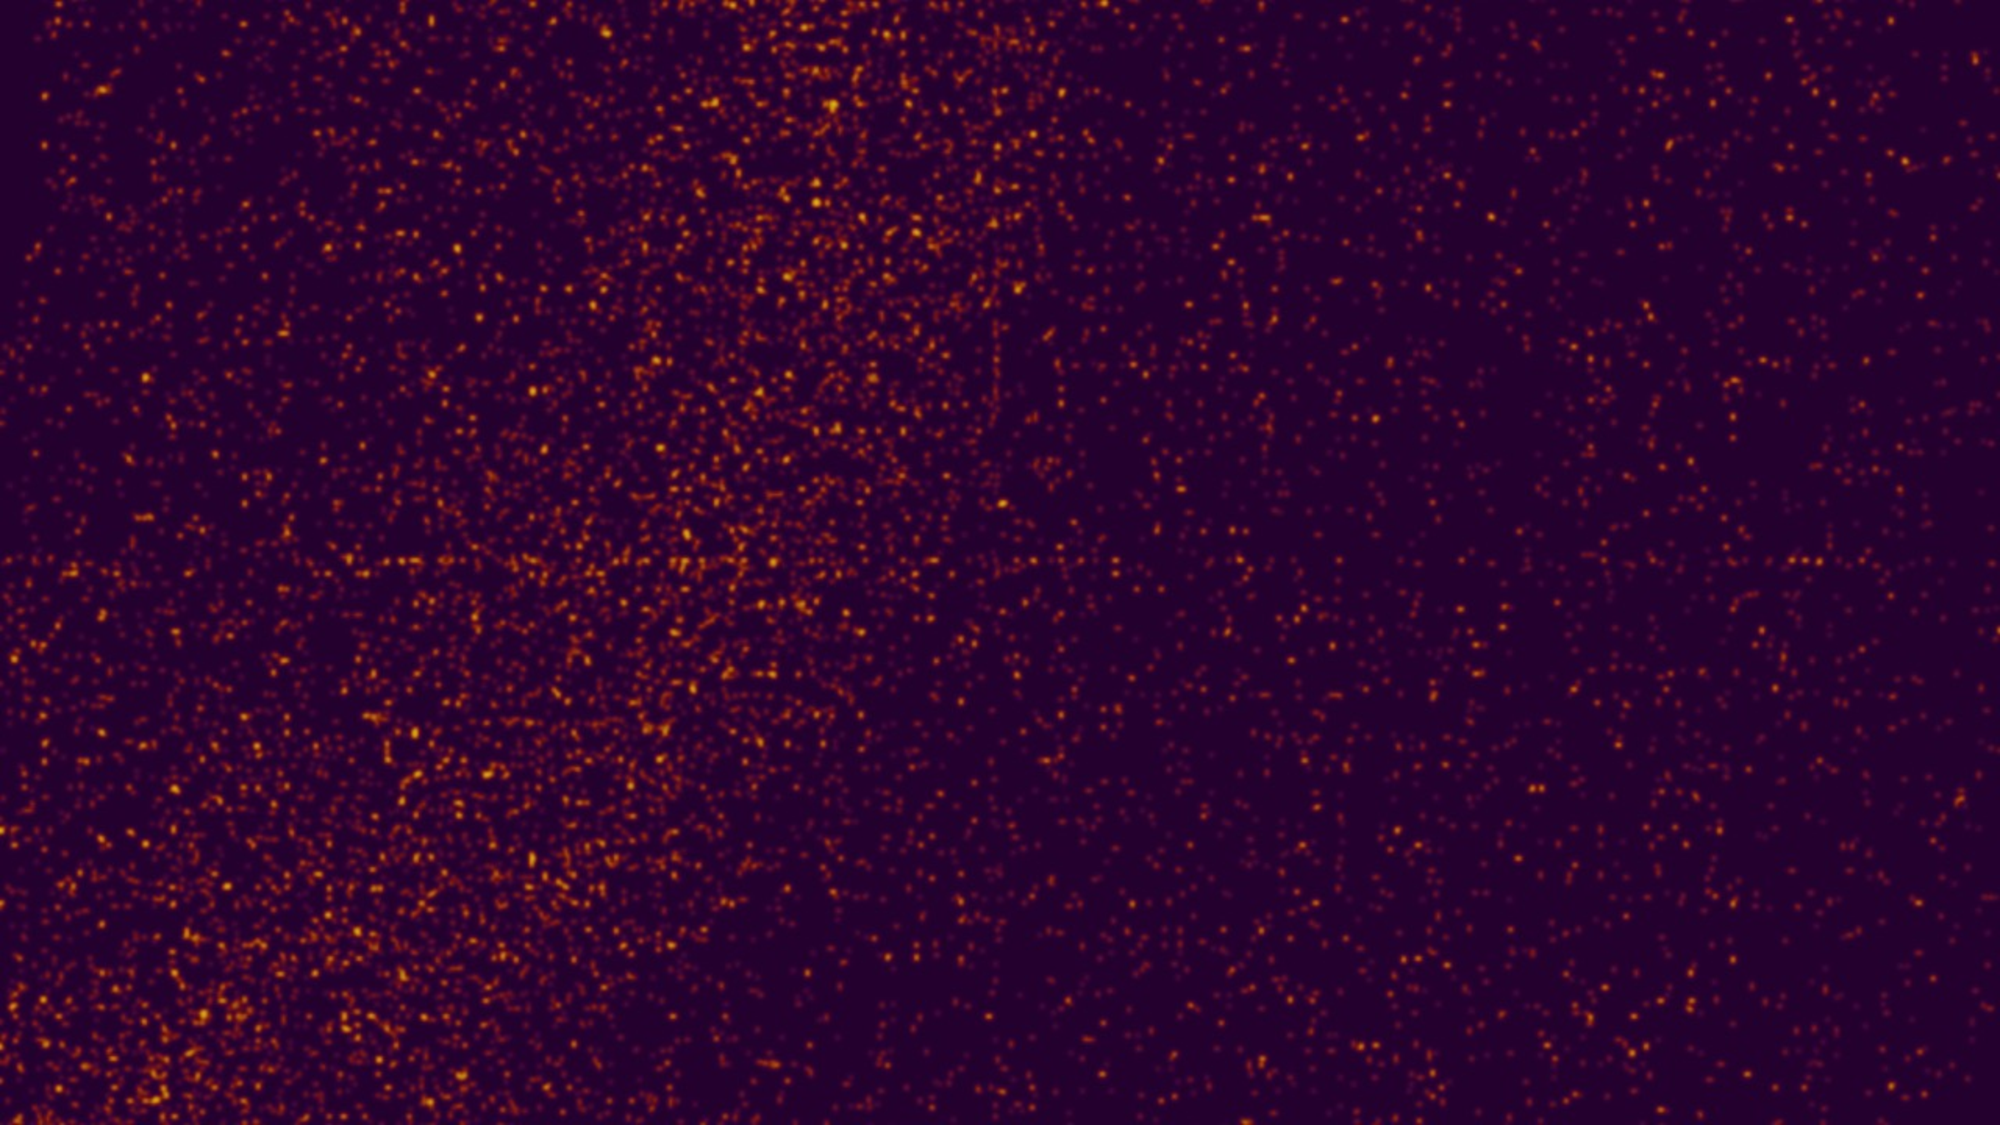
\includegraphics[width=1.2\linewidth]{./template/images/titlepage_background.pdf}}% Background/main image
    }
    \makeatletter
    \setbeamertemplate{title page}[default][left,colsep=-4bp] % align title page left
    \makeatother
    \setbeamerfont{title}{size=\@setfontsize\Huge{30}{20}}
    \setbeamercolor{title}{fg=white}
    \setbeamerfont{subtitle}{size=\@setfontsize\Huge{16}{12}}
    \setbeamercolor{subtitle}{fg=white}
    \setbeamercolor{author}{fg=white}
    \setbeamercolor{date}{fg=white}
    \setbeamercolor{institute}{fg=white}
    \setbeamertemplate{title page}{
        \vfill
        \begingroup
        \begin{groupcolumns}
            \hfill
            \begin{column}{0.65\textwidth}
                \usebeamertemplate{date}
                \usebeamertemplate*{title}
                \usebeamertemplate*{subtitle}
            \end{column}
            \begin{column}{0.35\textwidth}
                \usebeamertemplate*{titlegraphic}
            \end{column}
            \hfill
        \end{groupcolumns}
        \vspace{2pt}
        {\color{white}\hrule height 1pt}
        \usebeamertemplate{author}
        % \usebeamertemplate{institute}
        \vfill
        % Institutions at the bottom bar
        \vspace{10pt}
        \blackstrip{30pt}
        \vspace{-27pt}
        \includesvg[height=12pt]{./template/images/SLAC_TID_white.svg}
        {\color{white}\vrule width 0.1pt}
        \includesvg[height=12pt]{./template/images/TID_ID_IC.svg}
        \hfill
        \includesvg[height=12pt]{./template/images/Stanford_University.svg}
        {\color{white}\vrule width 0.1pt}
        \includesvg[height=12pt]{./template/images/DOE.svg}
        \vspace{4pt} % \vspace{-4pt}
        \endgroup
    }
}
\makeatother


% SloganTitleUnderline slide template
\makeatletter
\define@key{beamerframe}{SloganTitleUnderline}[true]{%
    \setbeamertemplate{frametitle}{%
        % \vskip-11.5pt % \vspace{-8.5pt}
        \vskip-11.5pt % \vspace{-8.5pt}
        \makebox[\textwidth]{
\includegraphics[width=\paperwidth]{./template/images/slogan.pdf}}
        \vskip-5pt%\vskip5.5pt 
        \usebeamerfont{frametitle}\huge\insertframetitle%
        \vphantom{g}% to avoid fluctuations per frame
        \vspace{3pt}% spacing between title text and horizontal line
        \hrule% 
        \vspace{-3pt}% adjust spacing after line
    }
    % \defaultfooter
}
\makeatother


% FloatingTitle (no underline) slide template
\makeatletter
\define@key{beamerframe}{FloatingTitle}[true]{%
    \setbeamertemplate{frametitle}{%
        \vskip-11.5pt % \vspace{-8.5pt}
        \makebox[\textwidth]{
\includegraphics[width=\paperwidth]{./template/images/slogan.pdf}}
        \vskip5.5pt
        \usebeamerfont{frametitle}\huge\insertframetitle%
        \vphantom{g}% to avoid fluctuations per frame
    }
    % \defaultfooter
}
\makeatother


% SectionTitlepage slide template
\makeatletter
\define@key{beamerframe}{SectionTitlepage}[true]{%
    \setbeamerfont{framesubtitle}{size=\@setfontsize\LARGE{12}{10}}
    \setbeamercolor{framesubtitle}{fg=stanford_black}%
    \setbeamertemplate{frametitle}{%
        \vskip-11.5pt % \vspace{-8.5pt}
        \makebox[\textwidth]{
\includegraphics[width=\paperwidth]{./template/images/slogan.pdf}}
        \vskip50pt
        {\color{stanford_black}\fontsize{35}{50}\selectfont\insertsectionnumber}
        \vskip6pt
        {\color{cardinal}\hrule height 0.5pt}
        \vskip15pt
        \usebeamerfont{frametitle}\Huge\insertframetitle%
        \vskip10pt
        \usebeamercolor[fg]{framesubtitle}\usebeamerfont{framesubtitle}\insertframesubtitle%
        \vphantom{g}% to avoid fluctuations per frame
    }
    % \defaultfooter
}
\makeatother


% TableOfContents (TOC) style
\setbeamertemplate{section in toc}[sections numbered]
% \setbeamerfont{section number projected}{size=\LARGE}
\setbeamerfont{section number projected}{size=\Large}
\setbeamercolor{section number projected}{bg=white,fg=black}

\setbeamertemplate{section in toc}{%
    \leavevmode\leftskip=4.75ex%1.75ex
  \llap{%
    \usebeamerfont*{section number projected}%
    \usebeamercolor[bg]{section number projected}%
    \vrule width2.25ex height1.85ex depth.4ex%
    \hskip-2.25ex%
    \hbox to2.25ex{\hfil\color{fg}\inserttocsectionnumber.\hfil}}%
\kern0.75ex\inserttocsection\par}

\makeatletter
\patchcmd{\beamer@sectionintoc}{\vskip1.5em}{\vskip0.5em}{}{}
% \patchcmd{\beamer@sectionintoc}{\vfill}{\vskip-0.2em}{}{} % reduce padding
% \patchcmd{\beamer@sectionintoc}{\vfill}{\vskip10pt}{}{} % reduce padding
\patchcmd{\beamer@sectionintoc}{\vfill}{\vskip1pt}{}{} % reduce padding
\makeatother






%%%%%%%%%%%%%%%%%%%%%%%%%%%%%%%%%%%%%%%%%%%%%%%%%%%%%%%%%%%%%%%%%%%%%%%%%%%%%%%%
%%%%%%%%%%%%%%%%%%%%%%%%%%%%%%%%%%%%%%%%%%%%%%%%%%%%%%%%%%%%%%%%%%%%%%%%%%%%%%%%
%%%%%%%%%%%%%%%%%%%%%%%%%%%%%%%%%%%%%%%%%%%%%%%%%%%%%%%%%%%%%%%%%%%%%%%%%%%%%%%%

\begin{document}


\begin{frame}[Titlepage, plain, noframenumbering]
\titlepage
\end{frame}

\begin{frame}{Introduction}
  \begin{columns}
      \begin{column}{0.5\textwidth}
        \begin{itemize}
            \item Llorenç Fanals-i-Batllori.
            \item BSc EE Universitat the Girona, Spain (9.52/10), MSc EE UPC Barcelona, Spain (9.69/10).
            \item Mixed-signal Design Verification Engineer at Apple, UK.
            \item Mixed-signal ASIC Design Engineer at SLAC/Stanford.
        \end{itemize}
      \end{column}
      \begin{column}{0.5\textwidth}
        \begin{figure} \centering
            
\includegraphics[width=0.8\textwidth]{./images/portrait_.jpeg}
        \end{figure}
      \end{column}
  \end{columns}
\end{frame}

\begin{frame}[SloganTitleUnderline]{Table of contents}
    \LARGE \tableofcontents%[section]
\end{frame}



%%%%%%%%%%%%%%%%%%%%%%%%%%%%%%%%%%%%%%%%%%%%%%%%%%%%%%%%%%%%%%%%%%%%%%%%%%%%%%%%
% 1: Cryogenic systems
%%%%%%%%%%%%%%%%%%%%%%%%%%%%%%%%%%%%%%%%%%%%%%%%%%%%%%%%%%%%%%%%%%%%%%%%%%%%%%%%
\section{Cryogenic systems}
\begin{frame}[SectionTitlepage]{Cryogenic systems}
\end{frame}
% Explain how a dilution refrigerator is wired and the need for power management
% 100 Ohms per DC wire, thermal load, quick simulation of how bad the power can be there, need for scaling

\begin{frame}{Dilution refrigerator}
\vspace{-0.4cm}
\begin{columns}[T]
  \begin{column}{0.55\textwidth}
      \begin{itemize}
        \item The power budget scales approximately as $\propto T^2$.
        \item Useful quantum computers need thousands or millions of qubits.
        \item $k_B T \ll \omega \hbar$ for quantum effects to show up \cite{Blais2021}.
        \item Cryo-CMOS at \SI{}{\m\K} temperatures needs to be show near zero static power consumption.
        \item The $4$-\SI{}{\K} is regarded as a suitable stage for more power-hungry cryo-CMOS \cite{Patra2018}.
      \end{itemize}
  \end{column}
  \begin{column}{0.4\textwidth}
    \begin{figure} \centering
        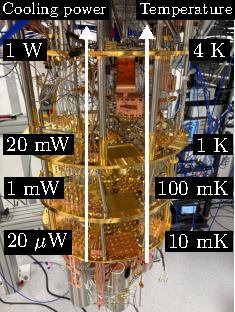
\includegraphics[width=0.9\textwidth]{./figures/dil_fridge.pdf}
    \end{figure}
  \end{column}
\end{columns}
\end{frame}

\begin{frame}{Cryo-CMOS motivation \cite{Patra2018}}
\vspace{-0.2cm}
    \begin{figure} \centering
        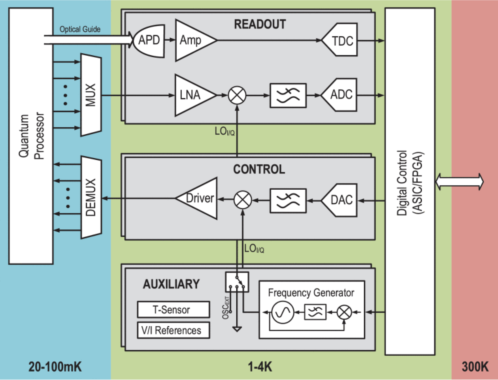
\includegraphics[width=0.65\textwidth]{./figures/patra2018.pdf}
    \end{figure}
\end{frame}

\begin{frame}{The need for power \cite{Patra2018}, adapted}
\vspace{-0.2cm}
    \begin{figure} \centering
        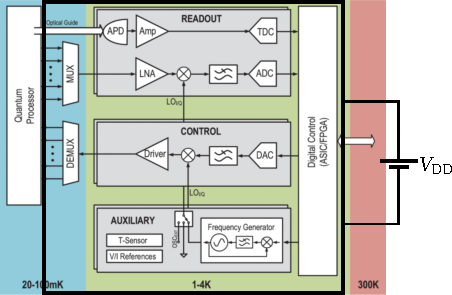
\includegraphics[width=0.75\textwidth]{./figures/patra2018_vdd.pdf}
    \end{figure}
\end{frame}

\begin{frame}{Equivalent model, DC}
\vspace{-0.2cm}
    \begin{figure} \centering
        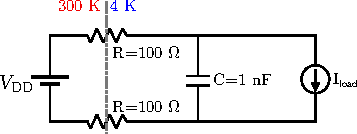
\includegraphics[width=0.5\textwidth]{./figures/wiring_model.pdf}
    \end{figure}
    Efficiency:
    \begin{equation}
        \eta \triangleq \frac{P_\text{out}}{P_\text{in}} = \frac{V_\text{DD} I_\text{load} - I_\text{load}^2 \cdot 2 R}{V_\text{DD} I_\text{load}} = 1 - \frac{ 2 I_\text{load} R}{V_\text{DD}} \ .
        \label{eq:efficiency}
    \end{equation}
    For $R = \SI{100}{\ohm}$, $V_\text{DD} = \SI{1}{\V}$, $I_\text{load} = \SI{1}{\mA}$, $\eta = 0.8$. The system stops working even for moderate loads!
    \begin{itemize}
        \item A single twisted pair is very resistive to minimize the heat load.
        \item Multiple twisted pairs in parallel are common, but this doesn't scale well.
    \end{itemize}
\end{frame}

\begin{frame}{Equivalent model, transient}
\vspace{-0.2cm}
    \begin{figure} \centering
        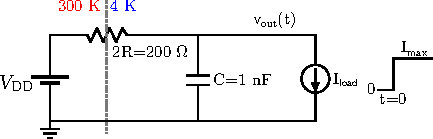
\includegraphics[width=0.6\textwidth]{./figures/wiring_model_transient.pdf}
    \end{figure}
    \begin{equation}
        \frac{V_\text{DD} - v_\text{out}(t)}{2 R} = C \frac{\partial v_\text{out}(t)}{\partial t} + i_\text{load}(t) \ .
    \end{equation}
    For a step on $i_\text{load} (t)$ from $0$ to $I_\text{max}$, 
    \begin{equation}
        v_\text{out}(t) = V_\text{DD} - 2 R I_\text{max} \left( 1 - e^{-\frac{t}{2RC}} \right) \ .
    \end{equation}
    For $R = \SI{100}{\ohm}$, $C = \SI{1}{\nF}$, $\tau = \SI{100}{\ns}$, slow!
\end{frame}

\begin{frame}{Equivalent model, transient}
\vspace{-0.6cm}
    \begin{equation}
        v_\text{out}(t) = V_\text{DD} - 2 R I_\text{max} \left( 1 - e^{-\frac{t}{2RC}} \right) \ .
    \end{equation}
    \begin{figure} \centering
        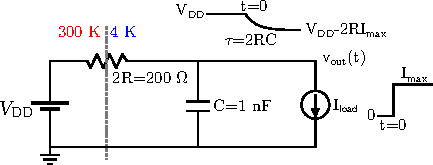
\includegraphics[width=0.6\textwidth]{./figures/wiring_model_transient_all.pdf}
    \end{figure}
    If we increase the number of twisted pairs by $N$,
    \begin{itemize}
        \item $v_\text{out}(t \rightarrow \infty)$ gets closer to $V_\text{DD}$.
        \item $\tau$ is kept constant.
    \end{itemize}
\end{frame}

\begin{frame}{+ LDO}
    \vspace{-0.2cm}
    \begin{figure} \centering
        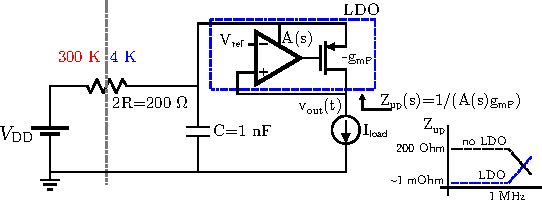
\includegraphics[width=0.8\textwidth]{./figures/wiring_model_ldo.pdf}
    \end{figure}
    \vspace{-0.3cm}
    The output impedance of the LDO is very low, leading to
    \begin{itemize}
        \item fast transients.
        \item A well-regulated voltage, $\epsilon \triangleq V_\text{ref} - V_\text{out} = \frac{V_\text{ref}}{1 + A(s) g_{mP} Z_\text{load}} = \frac{V_\text{ref}}{1 + T(s)}$.
    \end{itemize}
    System-wise, the efficiency $\eta$ is still poor. How to improve it?
\end{frame}

\begin{frame}{+ buck converter \cite{Faine2026}}
    \vspace{-0.2cm}
    \begin{figure} \centering
        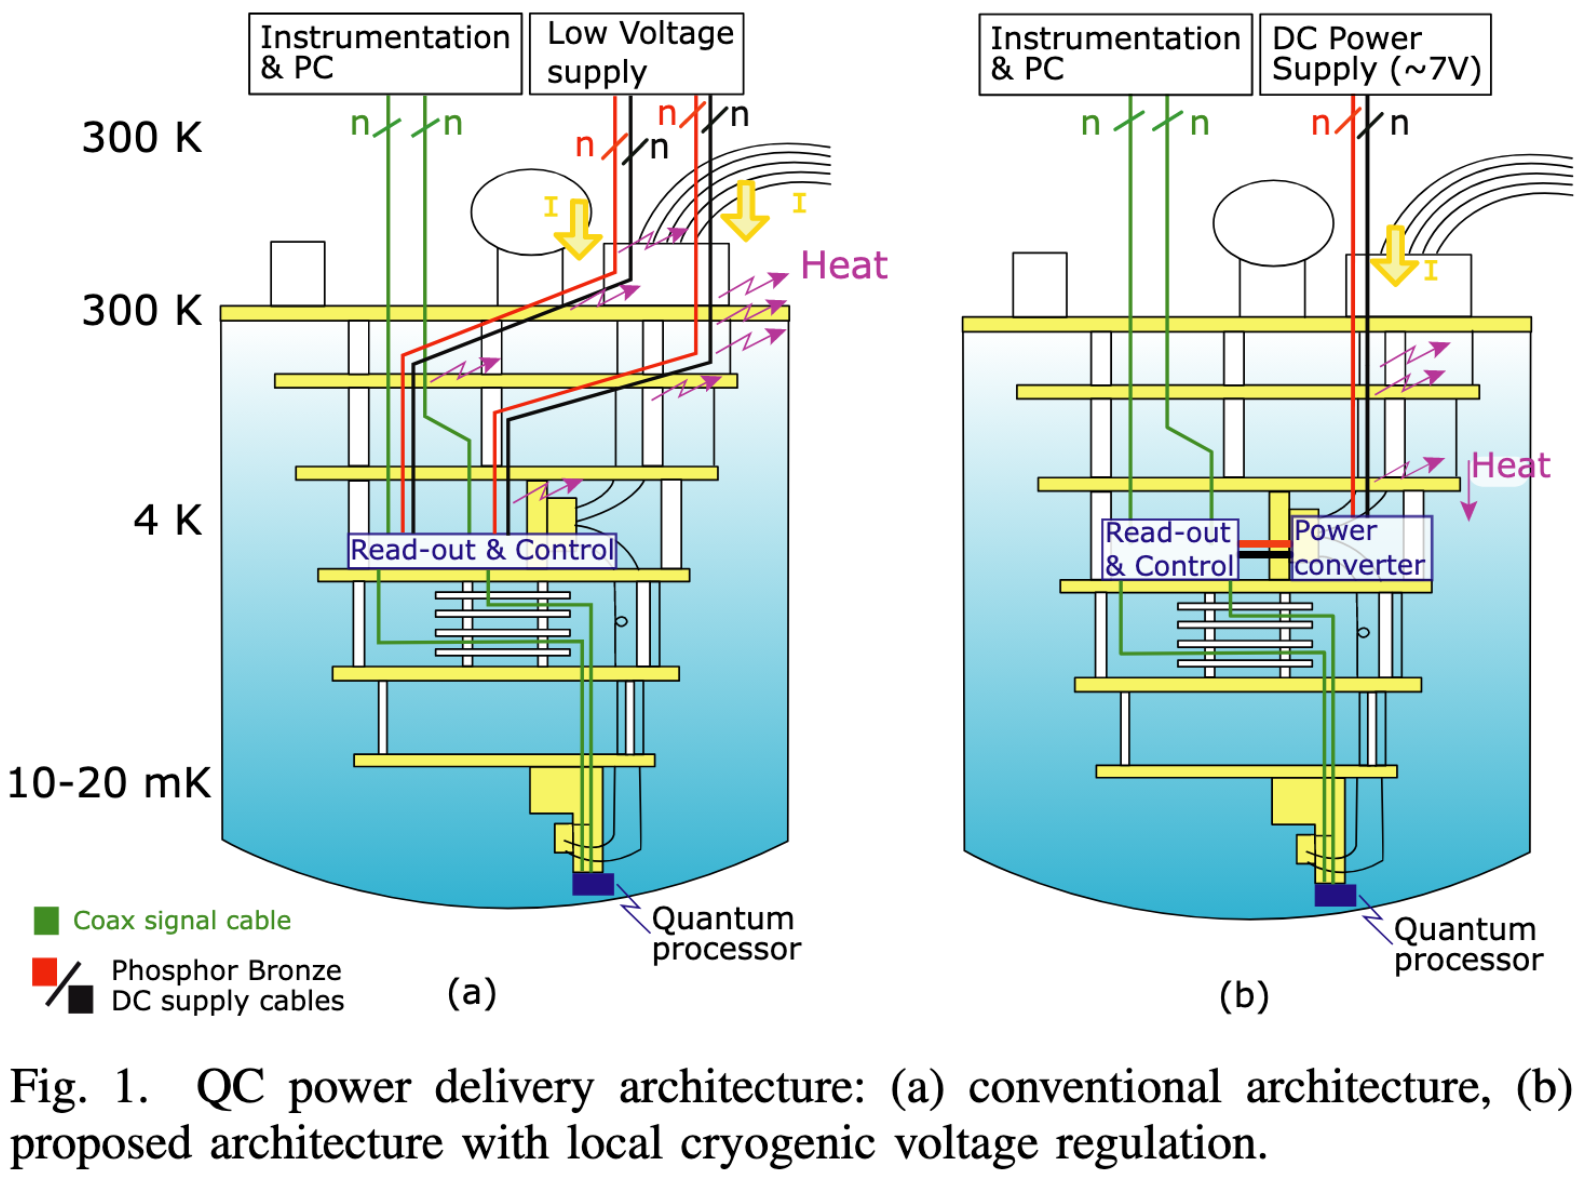
\includegraphics[width=0.65\textwidth]{./images/faine.png}
    \end{figure}
\end{frame}

\begin{frame}{+ buck converter}
    \vspace{-0.2cm}
    \begin{figure} \centering
        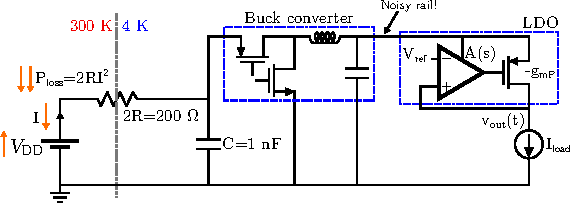
\includegraphics[width=0.8\textwidth]{./figures/wiring_model_buck_ldo.pdf}
    \end{figure}
    \vspace{-0.2cm}
    \begin{itemize}
        \item $V_\text{DD}$ is maximized to minimize the supply current. $P_\text{loss} = 2R \cdot I^2$ is minimized.
        \item An LDO is mandatory to clean the buck output ripple voltage.
        \item Ubiquitous architecture, found in almost all batery-operated devices.
    \end{itemize}
\end{frame}



%%%%%%%%%%%%%%%%%%%%%%%%%%%%%%%%%%%%%%%%%%%%%%%%%%%%%%%%%%%%%%%%%%%%%%%%%%%%%%%%
% 2: MOS temperature behavior
%%%%%%%%%%%%%%%%%%%%%%%%%%%%%%%%%%%%%%%%%%%%%%%%%%%%%%%%%%%%%%%%%%%%%%%%%%%%%%%%
\section{MOS temperature behavior}
\begin{frame}[SectionTitlepage]{MOS temperature behavior}
\end{frame}
% Derivation of SS, gm/Id, small-signal approximation

\begin{frame}{MOS temperature behavior, $22$-\SI{}{\nm} FDSOI}
\vspace{-0.8cm}
\begin{columns}
    \begin{column}{0.175\textwidth}
      \begin{figure} \centering
          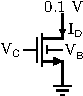
\includegraphics[width=0.9\textwidth]{./figures/mos_ss.pdf}
      \end{figure}
    \end{column}
    \begin{column}{0.8\textwidth}
    \begin{figure}[htpb] \centering
      \begin{tikzpicture}
        \begin{axis}[
            xlabel={$V_\text{GS}$ $\left[\SI{}{\V}\right]$},
            ylabel={$I_\text{DS}$ $\left[\SI{}{\A}\right]$},
            ymode=log,
            width=10cm,
            height=6cm,
            legend style={at={(0.98,0.02)}, anchor=south east, font=\small},
          ]                                                                
          \addplot+[mark=none, color=red] table [col sep=comma, x=Vgs_V, y=Ids_0Vbulk_A] {./datasets/SS_300K_1u1u_100mVds_1Vbulk.csv};
          \addlegendentry{\SI{300}{\K}, $V_\text{BS} = \SI{0}{\V}$}
          \addplot+[mark=none, color=red, dashed] table [col sep=comma, x=Vgs_V, y=Ids_1Vbulk_A] {./datasets/SS_300K_1u1u_100mVds_1Vbulk.csv};
          \addlegendentry{\SI{300}{\K}, $V_\text{BS} = \SI{1}{\V}$}
    
          \addplot+[mark=none, color=blue] table [col sep=comma, x=Vgs_V, y=Ids_0Vbulk_A] {./datasets/SS_4K_1u1u_100mVds_1Vbulk_fine.csv};
          \addlegendentry{\SI{4}{\K}, $V_\text{BS} = \SI{0}{\V}$}
          \addplot+[mark=none, color=blue, dashed] table [col sep=comma, x=Vgs_V, y=Ids_1Vbulk_A] {./datasets/SS_4K_1u1u_100mVds_1Vbulk_fine.csv};
          \addlegendentry{\SI{4}{\K}, $V_\text{BS} = \SI{1}{\V}$}
        \end{axis}                                                         
      \end{tikzpicture}
      % \caption{$I_{DS} \left(V_{GS}\right)$ of a $W=L=\SI{1}{\um}$ NMOS device with $V_{DS} = \SI{100}{\mV}$ at \SI{300}{\K} (PDK models) and \SI{4}{\K} (cryogenic models).}
      \label{fig:ss}
    \end{figure}
    \end{column}
\end{columns}
\vspace{-0.4cm}
$\SI{300}{\K} \rightarrow \SI{4}{\K}$ yields \cite{Beckers2018}
\begin{itemize}
    \item An increase in threshold voltage $\Delta V_\text{TH} \approx \SI{150}{\mV}$.
    \item An increase in mobility $\frac{\mu_\text{4 K}}{\mu_\text{300 K}} \approx 2.5$.
\end{itemize}
\end{frame}

\begin{frame}{MOS temperature behavior, $28$-\SI{}{\nm} bulk \cite{Beckers2020}}
% \vspace{-0.8cm}
      \begin{figure} \centering
          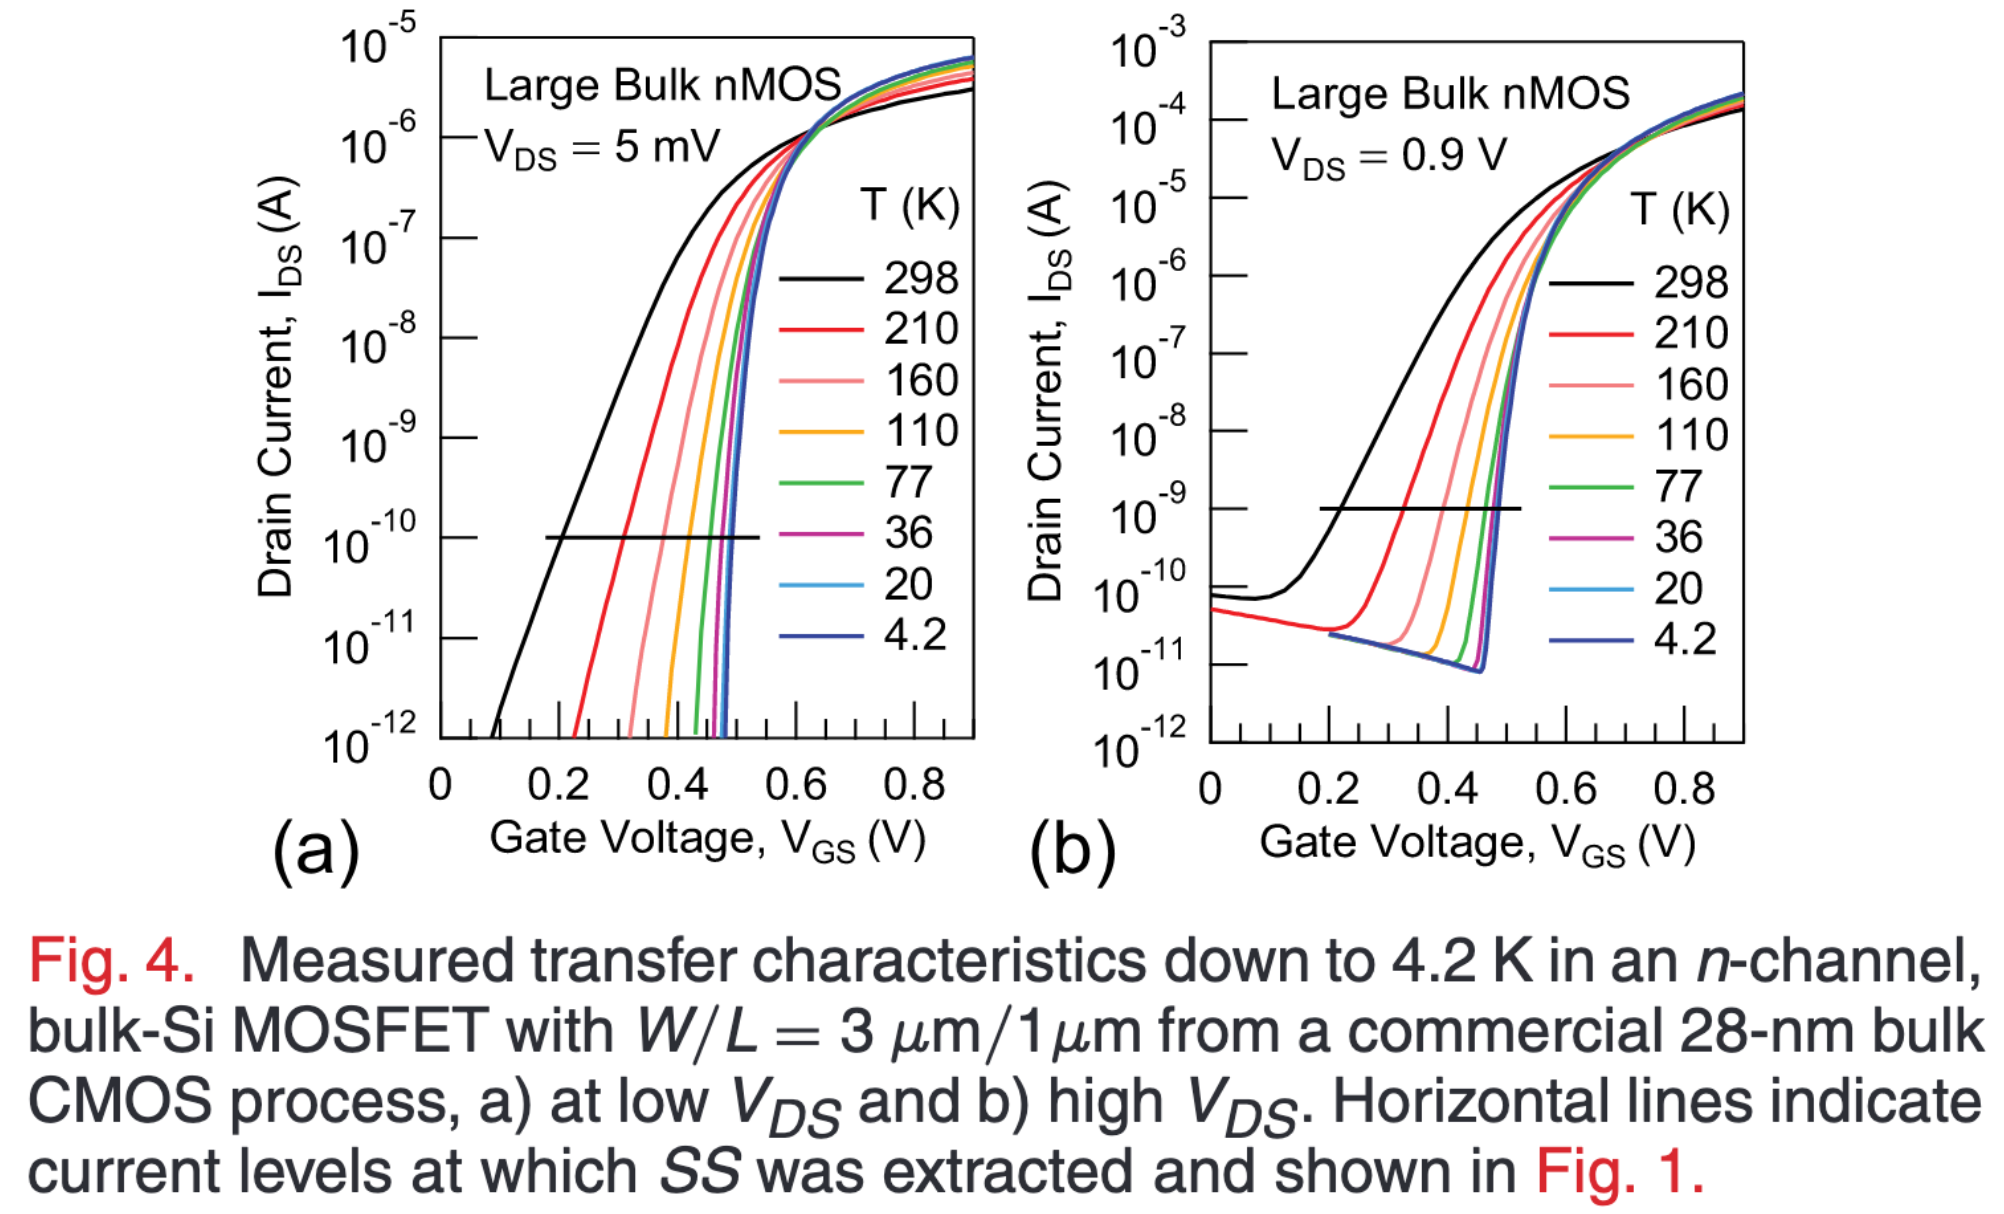
\includegraphics[width=0.8\textwidth]{./images/beckers2020.png}
      \end{figure}
\end{frame}

\begin{frame}{MOS temperature behavior, $28$-\SI{}{\nm} bulk \cite{Beckers2020}}
    \vspace{-0.2cm}
      \begin{figure} \centering
          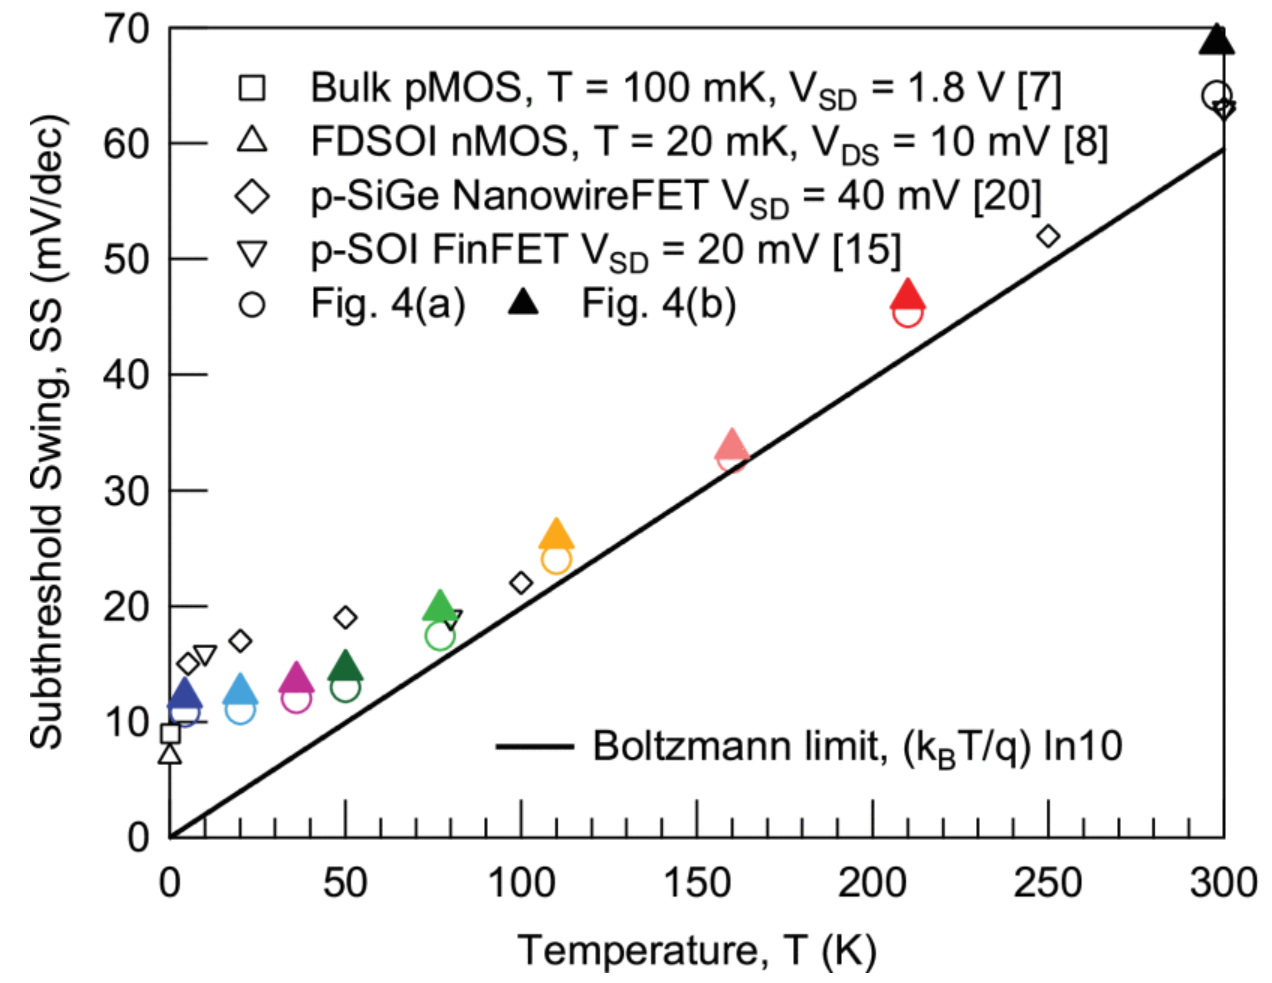
\includegraphics[width=0.5\textwidth]{./images/beckers2020_SS.png}
      \end{figure}
    \vspace{-0.4cm}
      \begin{itemize}
          \item As long as superconductivity is not achieved, MOS behaves the same below \SI{35}{\K}.
          \item For calculations, take $T = \SI{35}{\K}$ as a saturation temperature.
      \end{itemize}
\end{frame}

\begin{frame}{MOS in weak inversion}
    In weak inversion,
\begin{equation}
    I_\text{DS,wi} = I_\text{D0} \frac{W}{L} e^{V_{GS} / \left(n k_B T / q\right)} \ ,
    \label{eq:Id_wi}
\end{equation}
where
\begin{itemize}
    \item $I_{DO} \propto e^{-V_\text{TH} / \left(n k_B T / q\right)}$, take it as a constant.
    \item $W, L$: transistor effective width and length, respectively.
    \item $n(T)$: subthreshold slope factor, $\sim 1.2$ for FDSOI and $1.4$ for bulk, increases at cryo.
    \item $k_B = \SI{1.38e-23}{\m\squared\kg\s\tothe{-2}\K\tothe{-1}}$: Boltzmann's constant.
    \item $T$: temperature, in \SI{}{\K}.
    \item $q = \SI{1.6e-19}{\C}$: charge of an electron.
\end{itemize}
\end{frame}

\begin{frame}{MOS WI to SI transition \cite{Sansen2006}}
In weak inversion,
\begin{equation}
    I_\text{DS,wi} = I_\text{D0} \frac{W}{L} e^{V_{GS} / \left(n k_B T / q\right)} \ , \ \frac{g_{m\text{,wi}}}{I_\text{DS,wi}} = \frac{1}{n k_B T / q} = \frac{\ln(10)}{SS}  \ .
\end{equation}
In strong inversion,
\begin{equation}
    I_\text{DS,si} \approx \mu_N C_{ox} \frac{W}{L} \left(V_\text{GS} - V_\text{TH}\right)^2 \left(1 + \lambda V_\text{DS} \right) \ , \ \frac{g_{m\text{,si}}}{I_\text{DS,si}} = \frac{2}{V_\text{GS} - V_\text{TH}} \ .
\end{equation}
The transition is at $ \frac{g_{m\text{,wi}}}{I_\text{DS,wi}} = \frac{g_{m\text{,si}}}{I_\text{DS,si}}$:
\begin{equation}
    \left( V_\text{OD} \right)_t \triangleq \left( V_\text{GS} - V_\text{TH} \right)_t = 2 n \frac{k_B T}{q} \ .
\end{equation}
\vspace{-0.6cm}
\begin{itemize}
    \item $\left( V_\text{OD} \right)_t$ = \SI{72}{\mV} at \SI{300}{\K} $\rightarrow$ $V_\text{OD} = \SI{200}{\mV}$ is taken for strong inversion.
    \item $\left( V_\text{OD} \right)_t$ = \SI{8.4}{\mV} at \SI{4}{\K} (assuming saturation at \SI{35}{\K}) $\rightarrow$ can achieve strong inversion with small $V_\text{OD}$, but be careful about $V_\text{TH}$ mismatch!
\end{itemize}
\end{frame}


\begin{frame}{$g_m / I_\text{DS}$}
    \vspace{-0.4cm}
    \begin{figure}[htpb] \centering
      \begin{tikzpicture}
        \begin{axis}[
            xlabel={$I_\text{DS}$ $\left[\SI{}{\A}\right]$},
            ylabel={$g_m / I_\text{DS}$ $\left[\SI{}{\per\V}\right]$},
            xmode=log,
            width=10cm,
            height=6cm,
            grid=both,
            minor tick num=4,
            major grid style={gray!50, thin},
            minor grid style={gray!20, very thin},
            title={$22$-\SI{}{\nm} FDSOI, Semiwise models, $W=L=\SI{1}{\um}$ NMOS},
            title style={yshift=-0.3cm},
            legend style={at={(0.98,0.98)}, anchor=north east, font=\small},
          ]                                                                
          \addplot+[mark=none, color=blue] table [col sep=comma, x=Id_A, y=gmId_1perV] {./datasets/gmId_22nm_4K_Vbulk0V.csv};
          \addlegendentry{\SI{4}{\K}}
          \addplot+[mark=none, color=red] table [col sep=comma, x=Id_A, y=gmId_1perV] {./datasets/gmId_22nm_300K_Vbulk0V.csv};
          \addlegendentry{\SI{300}{\K}}
        \end{axis}                                                         
      \end{tikzpicture}
    \end{figure}
%    
    \vspace{-0.6cm}
    \begin{itemize}
        \item In \cite{Beckers2020}, $\min(SS) = \SI{10}{\mV}$/dec $\rightarrow$ $g_m / I_\text{DS} = 230 \SI{}{\per\V}$ and $g_m / I_\text{DS} \approx \SI{500}{\per\V}$ at low $I_\text{DS}$. 
        \item Large $g_m / I_\text{DS}$ means a high current efficiency, but a slow speed.
    \end{itemize}
\end{frame}


\begin{frame}{Small-signal validity in weak inversion}
    $g_m = \frac{\partial I_\text{DS}}{\partial V_\text{GS}}$ is a linearization around the operating point.

    How much error does this approximation yield?

    % Recall,
    \begin{equation}
        I_\text{DS,wi} = I_\text{D0} \frac{W}{L} e^{V_{GS} / \left(n k_B T / q\right)} \ .
    \end{equation}
    A Taylor expansion of $f(x)$ around $x_0$ is
    \begin{equation}
        f(x) \approx f(x_0) + \frac{\partial f(x_0)}{\partial x^1} \frac{(x - x_0)^1}{1!} + \frac{\partial f(x_0)}{\partial x^2} \frac{(x - x_0)^2}{2!} + \frac{\partial f(x_0)}{\partial x^3} \frac{(x - x_0)^3}{3!} + ... \ .
    \end{equation}
    We can think in terms of absolute and relative errors:
    \begin{equation}
        \epsilon_\text{abs} (x) \triangleq \left( f(x_0) + \frac{\partial f(x)}{\partial x^1} \frac{(x - x_0)^1}{1!} \right) - f(x) \ .
    \end{equation}
    \begin{equation}
        \epsilon_\text{rel} (x) \triangleq \frac{|\epsilon_\text{abs}(x)|}{f(x_0) + \frac{\partial f(x)}{\partial x^1} \frac{(x - x_0)^1}{1!}} \ .
    \end{equation}
\end{frame}

\begin{frame}{Small-signal validity in weak inversion}
  \vspace{-0.3cm}
  \begin{figure}[htpb] \centering
  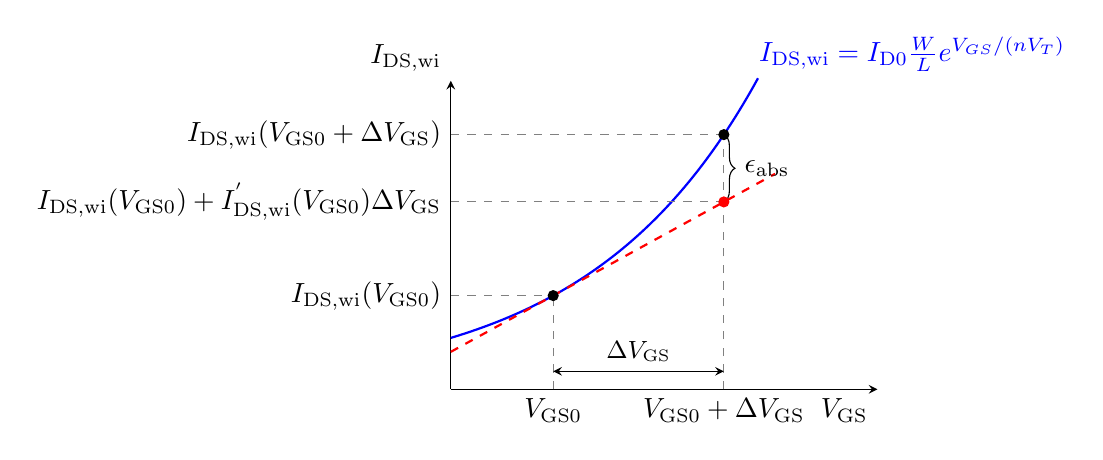
\begin{tikzpicture}
    \pgfmathsetmacro{\xo}{0.6}              % expansion point
    \pgfmathsetmacro{\dx}{1}            % step Delta x
    \pgfmathsetmacro{\xi}{\xo+\dx}        % x0 + Delta x
    \pgfmathsetmacro{\yo}{exp(\xo)}       % f(x0) = f'(x0) = e^{x0}
    \pgfmathsetmacro{\yt}{\yo*(1+\dx)}    % tangent value at x0 + Delta x
    \pgfmathsetmacro{\yi}{exp(\xi)}       % true value at x0 + Delta x
    \begin{axis}[
        width=7cm, height=5.5cm,
        xmin=0, xmax=2.5, ymin=0, ymax=6,
        axis lines=middle,
        xtick=\empty, ytick=\empty,
        clip=false,
        xlabel={$V_\text{GS}$},
        ylabel={$I_\text{DS,wi}$},
        xlabel style={anchor=north east},
        ylabel style={anchor=south east},
      ]
      % the function
      \addplot[blue, thick, domain=0:1.8, samples=200] {exp(x)};
      \node[blue, anchor=south west] at (axis cs:1.75, 6.0) {$I_\text{DS,wi} = I_\text{D0} \frac{W}{L} e^{V_{GS} / \left(n V_T\right)}$};

      % tangent at x0, clipped to x >= 0
      \addplot[red, thick, dashed, domain=0:\xi+0.3, samples=2] {\yo*(1 + x - \xo)};

      % drop lines to the x axis
      \draw[gray, dashed] (axis cs:\xo,0) -- (axis cs:\xo,\yo);
      \draw[gray, dashed] (axis cs:\xi,0) -- (axis cs:\xi,\yi);
      % drop lines to the y axis
      \draw[gray, dashed] (axis cs:0,\yo) -- (axis cs:\xo,\yo);
      \draw[gray, dashed] (axis cs:0,\yt) -- (axis cs:\xi,\yt);
      \draw[gray, dashed] (axis cs:0,\yi) -- (axis cs:\xi,\yi);

      % points
      \addplot[only marks, mark=*, mark size=1.8pt, black]
        coordinates {(\xo,\yo) (\xi,\yi)};
      \addplot[only marks, mark=*, mark size=1.8pt, red]
        coordinates {(\xi,\yt)};

      % x axis labels
    \node[anchor=north] at (axis cs:\xo,0) {$V_\text{GS0}$};
    \node[anchor=north] at (axis cs:\xi,0) {$V_\text{GS0}+\Delta V_\text{GS}$};
    \draw[<->, >=stealth] (axis cs:\xo,0.35) -- (axis cs:\xi,0.35)
    node[midway, above, font=\small] {$\Delta V_\text{GS}$};

      % y axis labels
    \node[anchor=east] at (axis cs:0,\yo) {$I_\text{DS,wi} (V_\text{GS0})$};
    \node[anchor=east] at (axis cs:0,\yt) {$I_\text{DS,wi} (V_\text{GS0}) + I_\text{DS,wi}^{'} (V_\text{GS0}) \Delta V_\text{GS} $};
    \node[anchor=east] at (axis cs:0,\yi) {$I_\text{DS,wi} (V_\text{GS0} + \Delta V_\text{GS})$};

      % absolute error brace
      \draw[decorate, decoration={brace, amplitude=4pt}]
        (axis cs:\xi,\yi) -- (axis cs:\xi,\yt)
        node[midway, anchor=west, xshift=4pt] {$\epsilon_\text{abs}$};
    \end{axis}
  \end{tikzpicture}
  \end{figure}

  \vspace{-0.5cm}
    \begin{equation}
        \epsilon_\text{abs} (V_\text{GS0} + \Delta V_\text{GS}) = I_\text{D0} \frac{W}{L} e^{V_\text{GS0}/(n V_T)} \left( 1 + \Delta V_\text{GS}/ (n V_T) - e^{\Delta V_\text{GS}/(n V_T)} \right) \ . 
    \end{equation}
    \begin{equation}
        \epsilon_\text{rel} (V_\text{GS0} + \Delta V_\text{GS}) = \frac{e^{\Delta V_\text{GS}/(n V_T)}}{1 + \Delta V_\text{GS}/(n V_T)} - 1 \ . 
    \end{equation}
\end{frame}


\begin{frame}{Small-signal validity in weak inversion, $\epsilon_\text{rel}$}
  \vspace{-0.2cm}
  \begin{figure}[htpb] \centering
  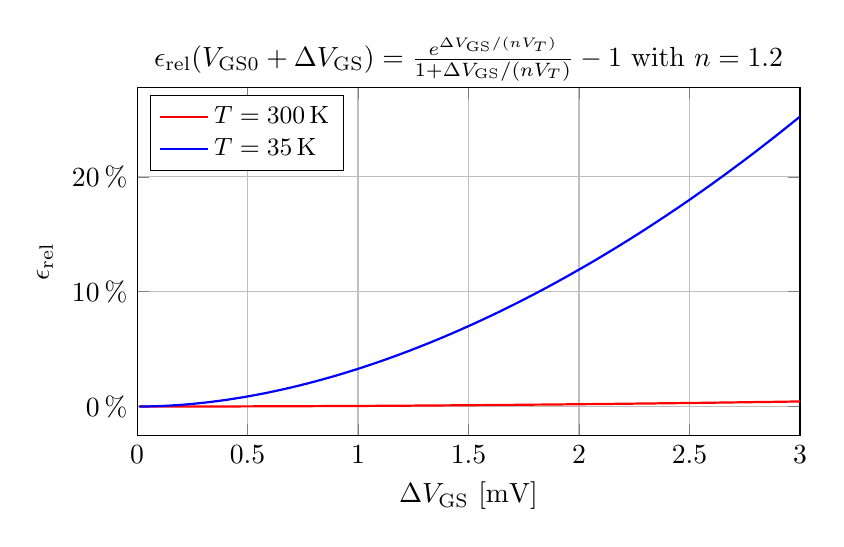
\begin{tikzpicture}
    \pgfmathsetmacro{\n}{1.2}
    \pgfmathsetmacro{\kq}{0.08617333}                 % k_B/q in mV/K
    \pgfmathsetmacro{\Vta}{\kq*300}                   % 25.85 mV
    \pgfmathsetmacro{\Vtb}{\kq*35}                    %  3.02 mV
    \begin{axis}[
        width=10cm, height=6cm,
        xmin=0, xmax=3,
        % ymode=log,
        xlabel={$\Delta V_\text{GS}$ $\left[\SI{}{\mV}\right]$},
        ylabel={$\epsilon_\text{rel}$},
        grid=both,
        major grid style={gray!50, thin},
        minor grid style={gray!20, very thin},
  title style={yshift=-0.25cm},
  yticklabel={\pgfmathprintnumber{\tick}\,\%},
  scaled y ticks=false,
  % y filter/.code={\pgfmathparse{##1*100}},
  y filter/.expression={y*100},
        legend style={at={(0.02,0.98)}, anchor=north west, font=\small},
        legend cell align=left,
        title={$\epsilon_\text{rel} (V_\text{GS0} + \Delta V_\text{GS}) = \frac{e^{\Delta V_\text{GS}/(n V_T)}}{1 + \Delta V_\text{GS}/(n V_T)} - 1$ with $n=1.2$},
      ]
      \addplot[red, thick, domain=0.01:3, samples=200]
        {exp(x/(\n*\Vta))/(1 + x/(\n*\Vta)) - 1};
      \addlegendentry{$T=\SI{300}{\K}$}

      \addplot[blue, thick, domain=0.01:3, samples=200]
        {exp(x/(\n*\Vtb))/(1 + x/(\n*\Vtb)) - 1};
      \addlegendentry{$T=\SI{35}{\K}$}
    \end{axis}
  \end{tikzpicture}
  \end{figure}

  \vspace{-0.3cm}
  $\epsilon_\text{rel} (1 n V_T) = \SI{35.9}{\percent}$, $\epsilon_\text{rel} (2 n V_T) = \SI{146}{\percent}$. At cryo, small-signal approximations fail quickly!
\end{frame}





%%%%%%%%%%%%%%%%%%%%%%%%%%%%%%%%%%%%%%%%%%%%%%%%%%%%%%%%%%%%%%%%%%%%%%%%%%%%%%%%
% 3: Literature review
%%%%%%%%%%%%%%%%%%%%%%%%%%%%%%%%%%%%%%%%%%%%%%%%%%%%%%%%%%%%%%%%%%%%%%%%%%%%%%%%
\section{Cryo LDO literature review}
% Equal1, Julich, and a few other LDOs

\begin{frame}[SectionTitlepage]{Cryo LDO literature review}
\end{frame}

% IBM
\begin{frame}{IBM \cite{underwood2023}}
    \vspace{-0.3cm}
    \begin{figure} \centering
        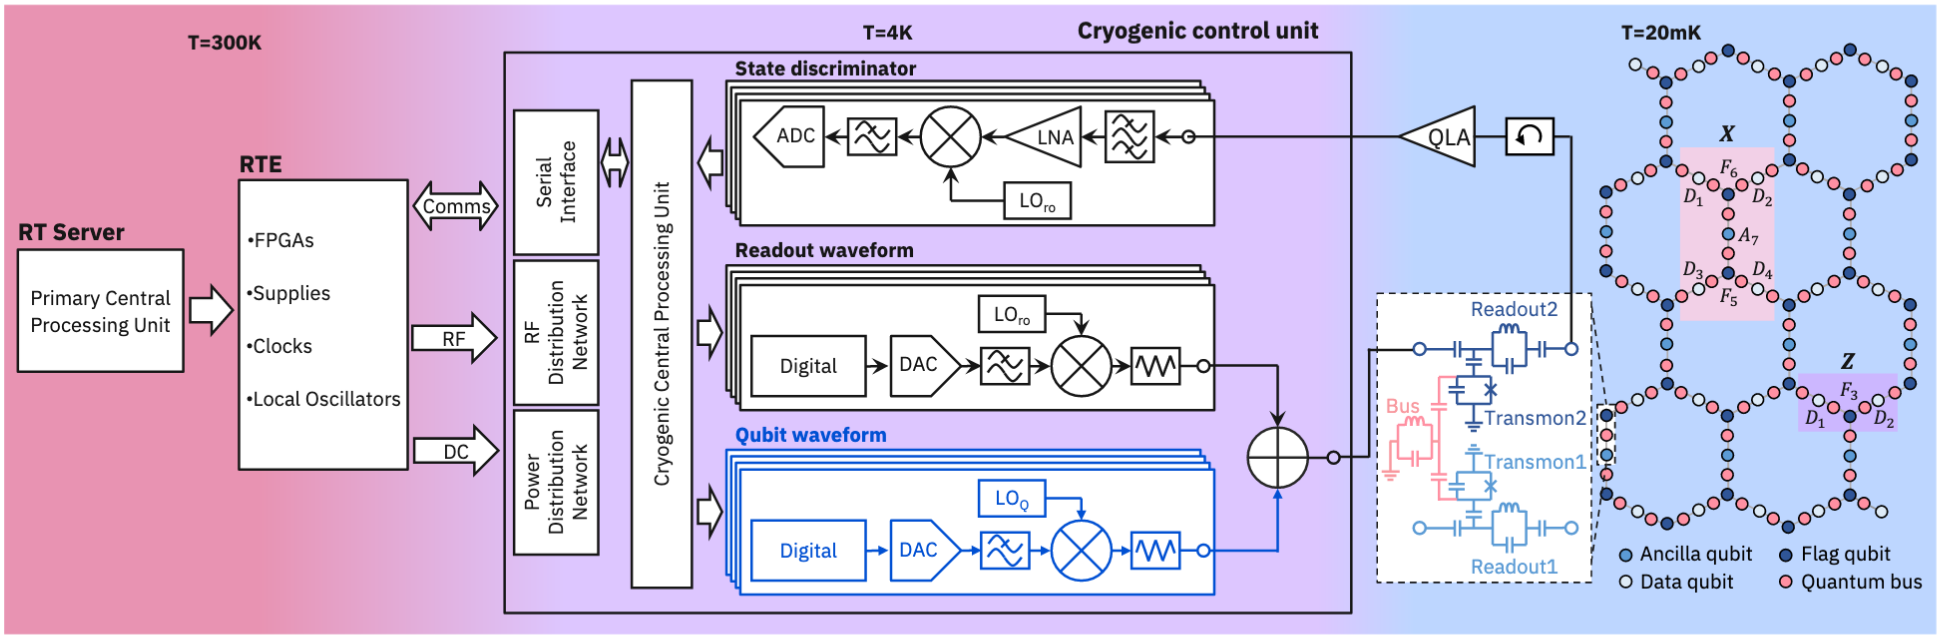
\includegraphics[width=0.95\textwidth]{./images/ibm_full.png}
    \end{figure}
\end{frame}

\begin{frame}{IBM \cite{underwood2023}}
    \vspace{-0.3cm}
    \begin{figure} \centering
        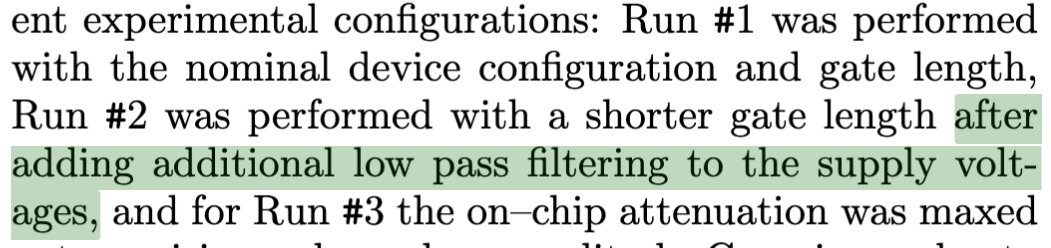
\includegraphics[width=0.5\textwidth]{./images/ibm_passive.png}
    \end{figure}
    \begin{figure} \centering
        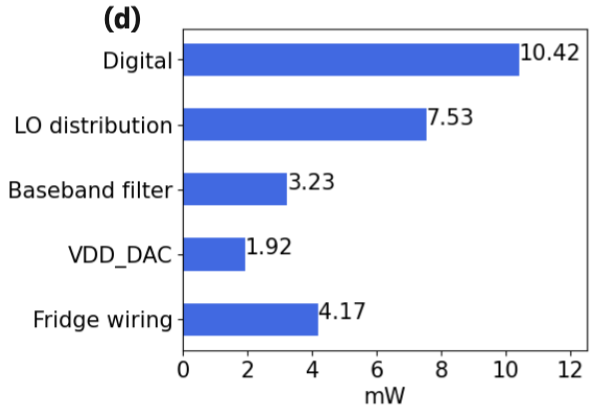
\includegraphics[width=0.4\textwidth]{./images/ibm_power.png}
    \end{figure}
   \vspace{-0.3cm}
   \begin{itemize}
    \item A passive approach is valid too.
    \item Wiring losses amount to \SI{4.17}{\mW}, amounting to \SI{16}{\percent} of the total power consumption.
   \end{itemize} 
\end{frame}


% Julich
\begin{frame}{Jülich \cite{ashok2025}}
    \vspace{-0.3cm}
    \begin{figure} \centering
        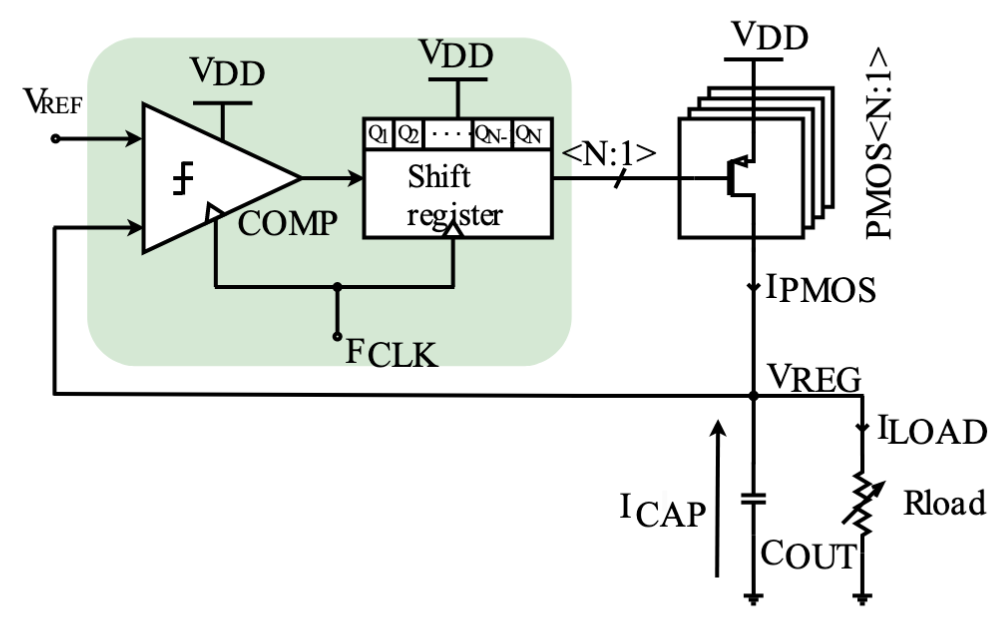
\includegraphics[width=0.6\textwidth]{./images/julich_digital.png}
    \end{figure}
   \vspace{-0.3cm}
   \begin{itemize}
    \item Pros versus A-LDO: lower dropout, higher efficiency $\eta$, portable to advanced nodes, robust. 
    \item Cons versus A-LDO: ripple in steady state, limited PSRR, speed (unless high power and ripple).
   \end{itemize} 
\end{frame}

\begin{frame}{Jülich \cite{ashok2025}}
    \vspace{-0.3cm}
    \begin{figure} \centering
        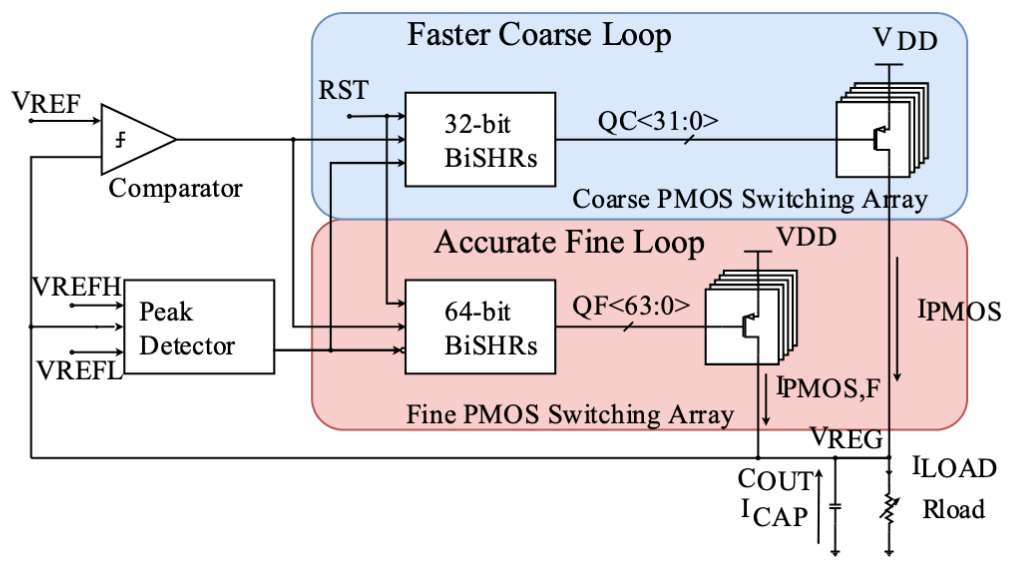
\includegraphics[width=0.6\textwidth]{./images/julich_digital_fine.png}
    \end{figure}
   \vspace{-0.3cm}
   \begin{itemize}
    \item Fine loop: enabled when $V_\text{out} \in \left[V_\text{REFL},\, V_\text{REFH}\right]$. 
    \item Coarse loop: enabled when $V_\text{out} \notin \left[V_\text{REFL},\, V_\text{REFH}\right]$. 
    \item $P_\text{cons} = \SI{325}{\uW}$ with a clock frequency of \SI{100}{\MHz}, in $22$-\SI{}{\nm} FDSOI.
   \end{itemize} 
\end{frame}

\begin{frame}{Jülich \cite{ashok2025}}
    \vspace{-0.3cm}
\begin{columns}
    \begin{column}{0.425\textwidth}
    \begin{itemize}
        \item How to improve the transient response? Lower the depth of the flop chain (sacrifice accuracy) or run with a faster clock (increase power consumption).
        \item There is always some ripple in steady state. Acceptable for digital loads, not for high-precision analog or mixed-signal.
    \end{itemize}
    \end{column}
    \begin{column}{0.55\textwidth}
      \begin{figure} \centering
        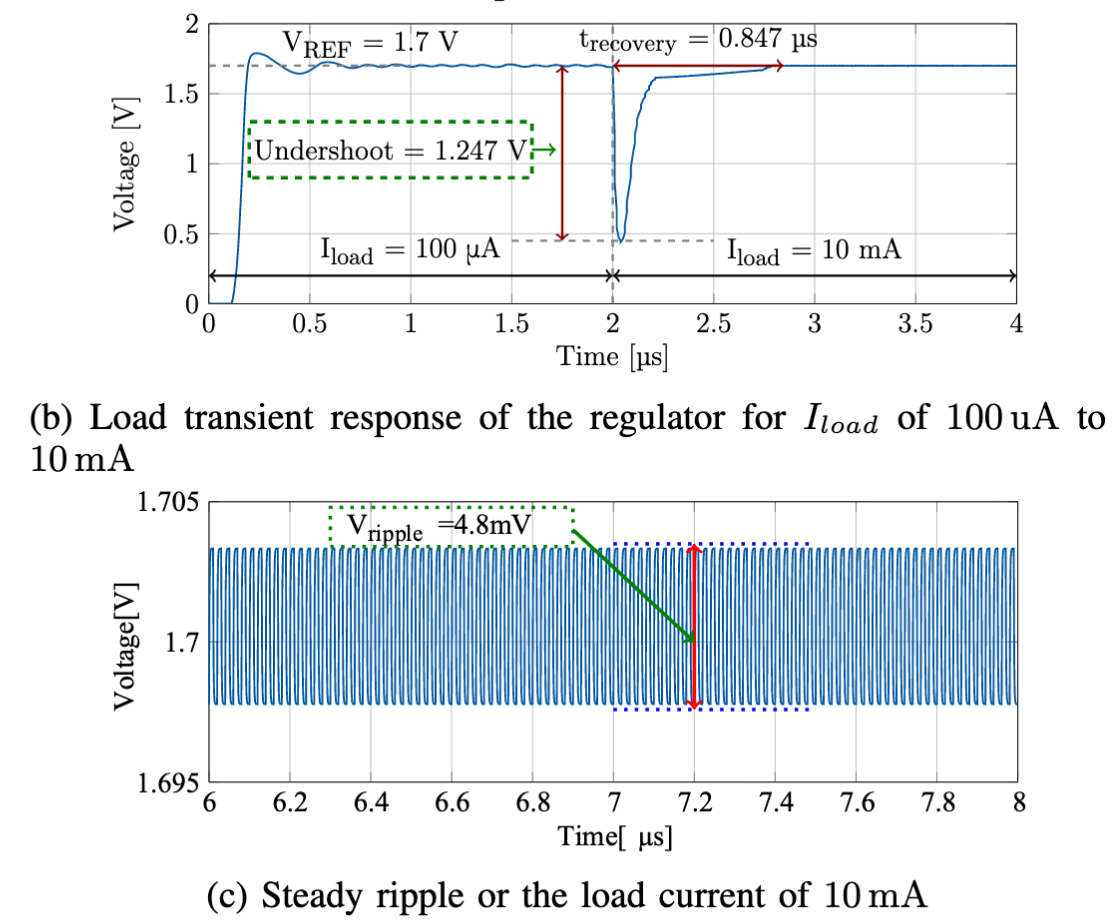
\includegraphics[width=0.99\textwidth]{./images/julich_transient.png}
      \end{figure}
    \end{column}
\end{columns}
\end{frame}



% Equal1
\begin{frame}{Equal1 \cite{Andrade2021}}
    \vspace{-0.3cm}
    \begin{figure} \centering
        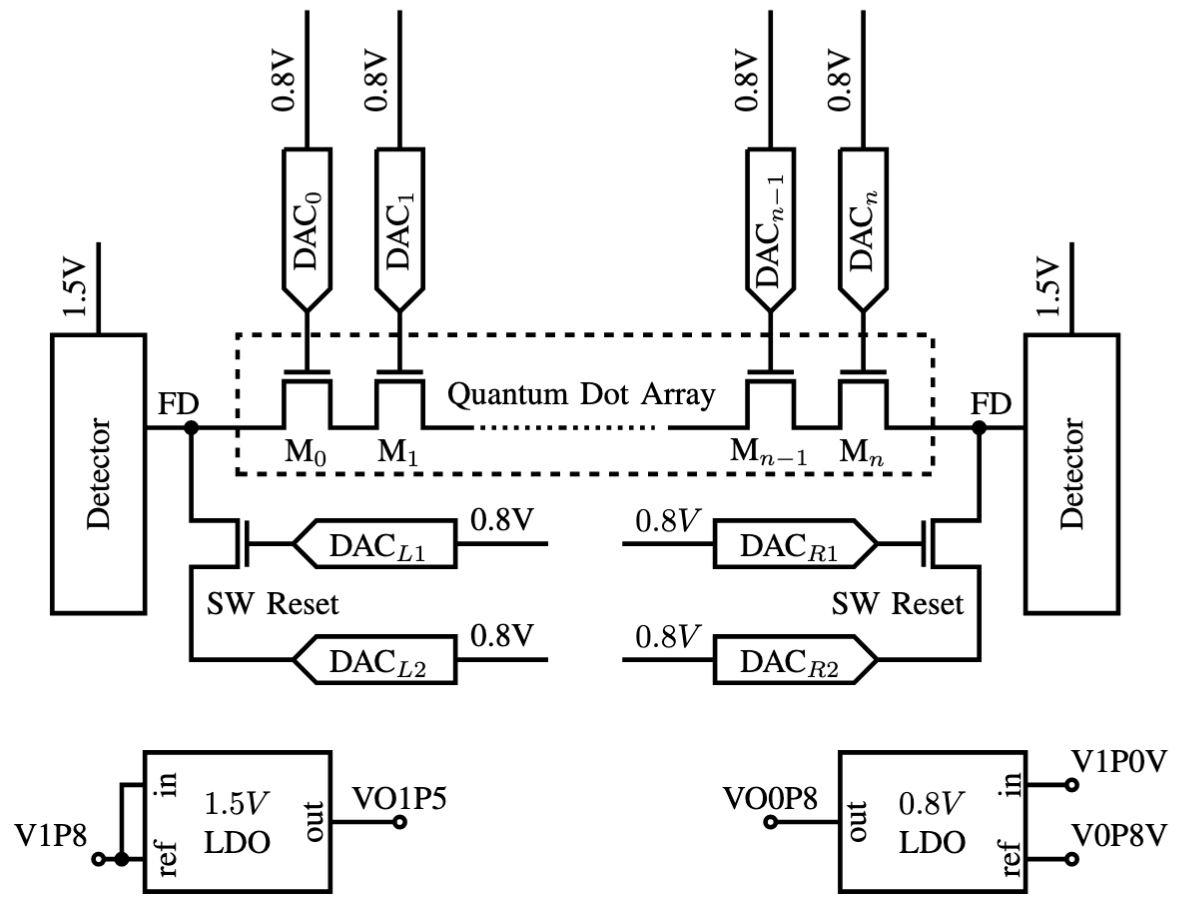
\includegraphics[width=0.5\textwidth]{./images/equal1_top.png}
    \end{figure}
   \vspace{-0.3cm}
   \begin{itemize}
    \item A DAC will never be better than its analog reference. Quiet and regulated rails are needed.
    \item \SI{1.5}{\V} for thick oxide devices, mostly used for analog circuits.
    \item \SI{0.8}{\V} for thin oxide devices, mostly used for digital circuits, to benefit from $P_\text{cons} \propto V_\text{DD}^2$.
   \end{itemize} 
\end{frame}

\begin{frame}{Equal1 \cite{Andrade2021}}
    \vspace{-0.3cm}
    \begin{figure} \centering
        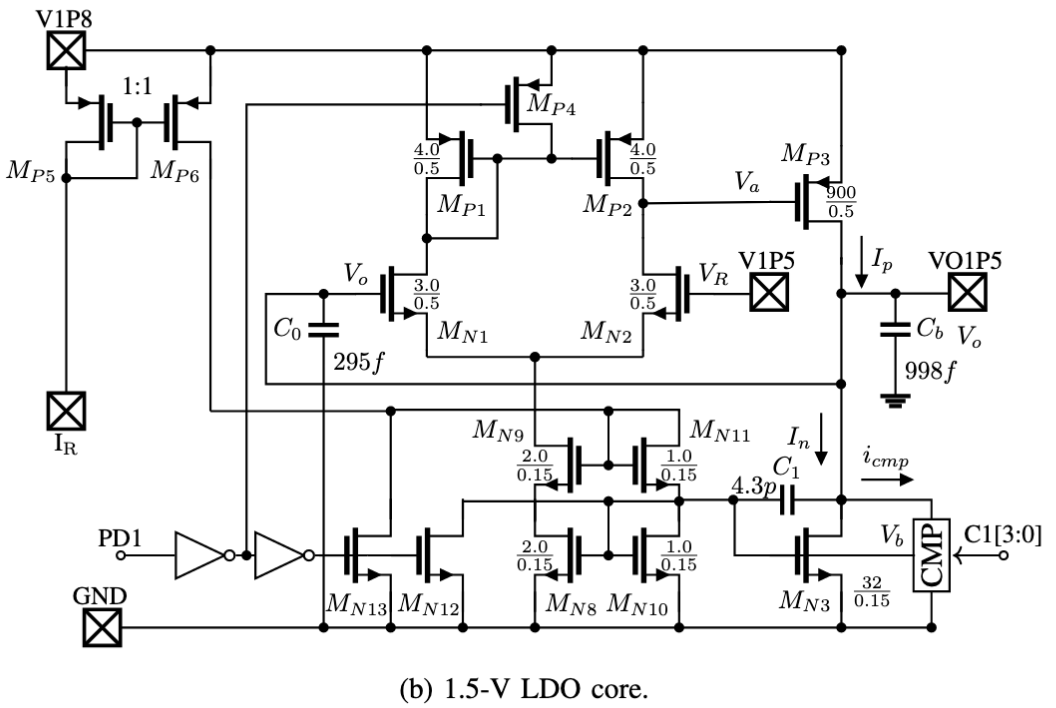
\includegraphics[width=0.55\textwidth]{./images/equal1_1p5V.png}
    \end{figure}
   \vspace{-0.3cm}
   \begin{itemize}
    \item PMOS pass device.
    \item There is enough headroom to afford cascode devices.
    \item CMP is a tunable compensation current to facilitate stability.
   \end{itemize} 
\end{frame}

\begin{frame}{Equal1 \cite{Andrade2021}}
    \vspace{-0.3cm}
    \begin{figure} \centering
        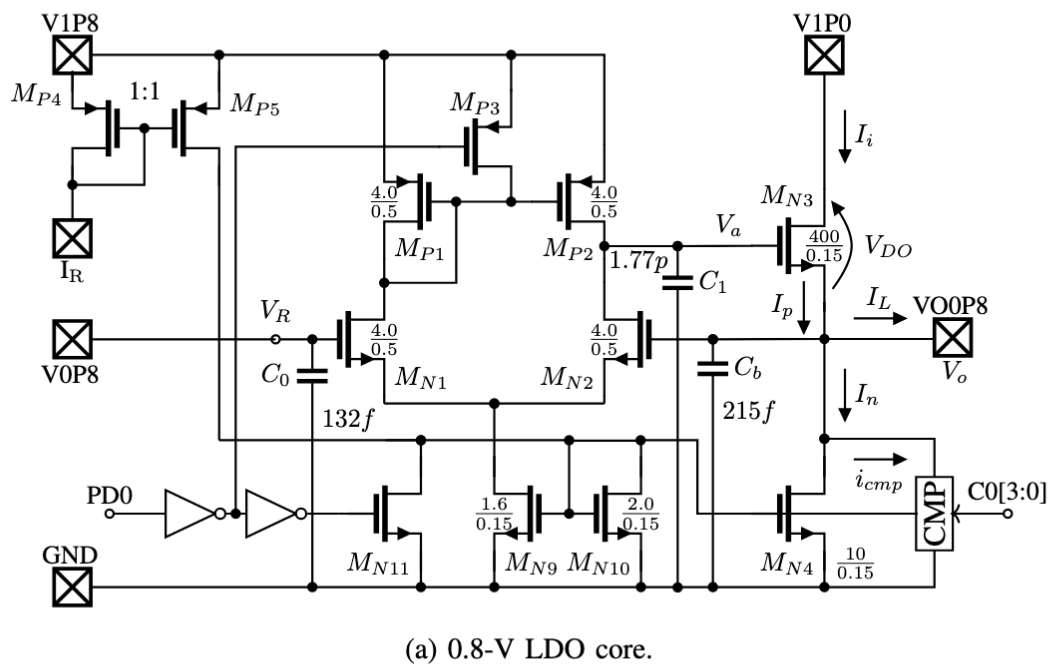
\includegraphics[width=0.55\textwidth]{./images/equal1_0p8V.png}
    \end{figure}
   \vspace{-0.3cm}
   \begin{itemize}
    \item NMOS pass device.
    \item The error amplifier is operated via \SI{1.8}{\V}, while the pass device sees \SI{1.0}{\V}.
    \item Only thick-oxide devices are used, with a minimum length of \SI{150}{\nm}. 
   \end{itemize} 
\end{frame}

\begin{frame}{Equal1 \cite{Andrade2021}}
    \vspace{-0.3cm}
    \begin{figure} \centering
        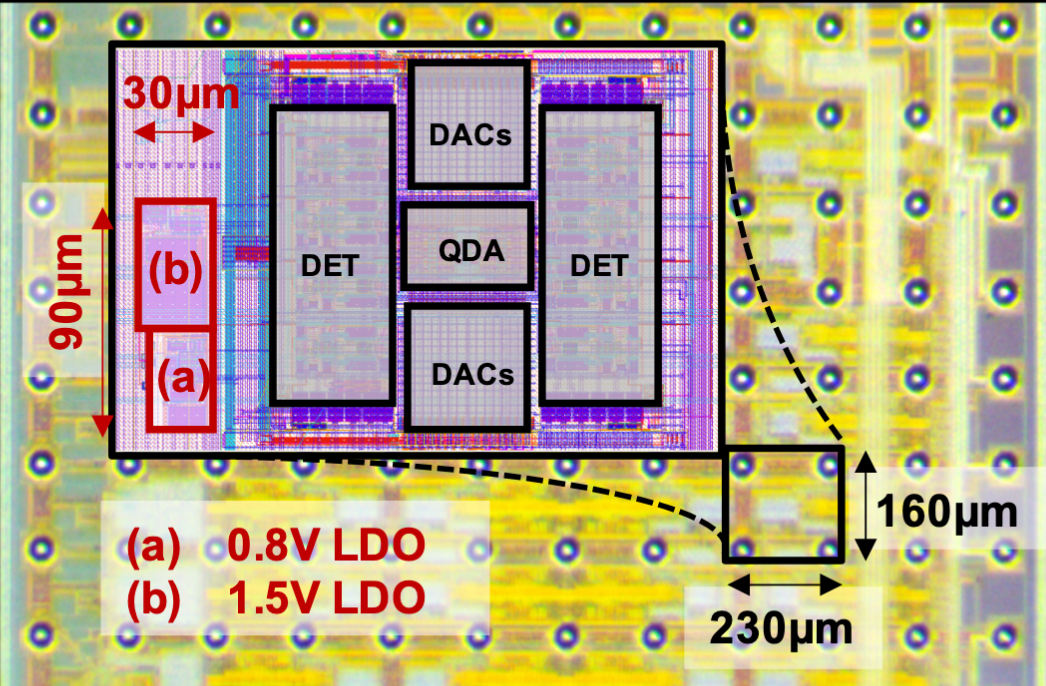
\includegraphics[width=0.55\textwidth]{./images/equal1_chip.png}
    \end{figure}
   \vspace{-0.3cm}
   \begin{itemize}
    \item LDOs are sitting next to the DACs and circuitry.
    \item Capless means low area overhead.
   \end{itemize} 
\end{frame}




%%%%%%%%%%%%%%%%%%%%%%%%%%%%%%%%%%%%%%%%%%%%%%%%%%%%%%%%%%%%%%%%%%%%%%%%%%%%%%%%
% 4: Design
%%%%%%%%%%%%%%%%%%%%%%%%%%%%%%%%%%%%%%%%%%%%%%%%%%%%%%%%%%%%%%%%%%%%%%%%%%%%%%%%
\section{Design}
\begin{frame}[SectionTitlepage]{Design}
\end{frame}
% Insights of our design

\begin{frame}{Design philosophy}
   \begin{itemize}
    \item Chose an analog LDO to have a ripple-free rail.
    \item Leverage weak inversion for a high $g_m/I_D$.
    \item Target $I_Q < \SI{2}{\uA}$ for compatibility with \SI{}{\milli\K} stages.
    \item Use dynamic large-signal circuits to aid transients.
    \item Accept the pass device dropout voltage as a tax to the power delivered to the load.
   \end{itemize} 
\end{frame}

\begin{frame}{Error amplifier + pass device}
\begin{figure}[H]
\centering
\begin{circuitikz}[american, transform shape, scale=0.7]
\ctikzset{tripoles/nmos/width=0.714286, tripoles/nmos/height=1.428571, tripoles/pmos/width=0.714286, tripoles/pmos/height=1.428571, tripoles/mos style/arrows, tripoles/pmos style/nocircle}
\draw (11,13) node[nmos] (M1) {}; \node[anchor=west] at (M1.text) {$\text{M}_{1}$};
\draw (15,13) node[nmos, xscale=-1] (M2) {}; \node[anchor=east] at (M2.text) {$\text{M}_{2}$};
\draw (13,10) node[nmos] (M3) {}; \node[anchor=west] at (M3.text) {$\text{M}_{3}$};
\draw (15,16) node[pmos] (M4) {}; \node[anchor=west] at (M4.text) {$\text{M}_{4}$};
\draw (11,16) node[pmos, xscale=-1] (M5) {}; \node[anchor=east] at (M5.text) {$\text{M}_{5}$};
\draw (7,10) node[nmos, xscale=-1] (M6) {}; \node[anchor=east] at (M6.text) {$\text{M}_{6}$};
\draw (13,17.5) node[vcc] {};
\draw (13,9) node[ground] {};
\draw (7,9) node[ground] {};
\draw (7,17.5) node[vcc] {};
\node at (13,16.5) {400n/3u};
\node at (8.5,9.5) {400n/8u};
\node at (10,10.5) {1:8};
\node at (13,13) {50x400n/400n};
\node at (8,12) {$V_\text{OD} = \SI{80}{\mV}$};
\draw (19,14.5) node[pmos] (M7) {}; \node[anchor=west] at (M7.text) {$\text{M}_{7}$};
\draw (19,17.5) node[vcc] {};
\node at (20,12) [circle, fill, inner sep=1.5pt] {};
\node at (20,12.5) {$V_\text{out}$};
\node at (20.5,15.5) {32x32x1u/20n};
\node at (13.5,18) {\SI{1}{\V}};
\node at (16.5,13) {$V_\text{ref}$};
\node at (16.5,14.75) {$V_\text{gpass}$};
\draw (M5.S) to[short] (11,17.5);
\draw (11,17.5) to[short] (15,17.5);
\draw (15,17.5) to[short] (M4.S);
\draw (M5.D) to[short] (M1.D);
\draw (M4.G) to[short] (M5.G);
\draw (12.5,16) to[short] (12.5,14.5);
\draw (12.5,14.5) to[short] (11,14.5);
\draw (M2.D) to[short] (M4.D);
\draw (M2.S) to[short] (15,11.5);
\draw (15,11.5) to[short] (11,11.5);
\draw (M1.S) to[short] (11,11.5);
\draw (13,11.5) to[short] (M3.D);
\draw (M3.G) to[short] (M6.G);
\draw (8.5,10) to[short] (8.5,11.5);
\draw (8.5,11.5) to[short] (7,11.5);
\draw (M6.D) to[short] (7,15);
\draw (7,17.5) to[isource,l=$\SI{100}{\nA}$] (7,15);
\draw (19,17.5) to[short] (M7.S);
\draw (M7.G) to[short] (15,14.5);
\draw (19,13) to[short] (19,12);
\draw (19,12) to[short] (20,12);
\draw (19,12) to[short] (15.5,12);
\draw (15.5,12) to[jump crossing] (14.5,12);
\draw (14.5,12) to[short] (11.5,12);
\draw (11.5,12) to[jump crossing] (10.5,12);
\draw (10.5,12) to[short] (9.5,12);
\draw (9.5,12) to[short] (9.5,13);
\draw (9.5,13) to[short] (M1.G);
\draw (19,13) to[short] (M7.D);
\node at (14.75,10) {$g_m/I_D = 25$};
\node at (13.5,15.5) {$g_m/I_D = 24$ };
\node at (9.5,14) {$g_m/I_D = 280$};
\end{circuitikz}
\end{figure}
\end{frame}



\begin{frame}{Frequency response}
    \begin{tikzpicture}

\pgfplotsset{
  width=6.5cm, height=5.6cm,
  xmode=log, xlabel={Frequency [\si{\hertz}]},
  grid=both, grid style={gray!25},
  tick label style={font=\small}, label style={font=\small},
  legend style={font=\small, cells={anchor=west}, draw=gray!50},
  title style={yshift=-1.2ex, font=\small},
  every axis plot/.append style={line width=0.9pt},
  xmin=1, xmax=1e9, xtick={1e0,1e2,1e4,1e6,1e8}, minor xtick={1e1,1e3,1e5,1e7,1e9},
}

% ---------------- loop gain: magnitude (left axis) + phase (right axis) ----------------
\begin{axis}[
  name=loop, xmode=log,
  title={Loop gain (light load)},
  ylabel={$|T|$ [\si{\deci\bel}]}, ymin=-60, ymax=100, ytick={-60,-40,-20,0,20,40,60,80,100},
  axis y line*=left,
  legend style={font=\small, at={(0.03,0.06)}, anchor=south west, draw=gray!50},
]
\addplot[blue] table[x=f_hz, y=loop_db, col sep=comma] {./datasets/ac_response.csv};
\addlegendentry{magnitude}
\addlegendimage{red, dashed}
\addlegendentry{phase, PM $=\SI{61.2}{\degree}$}
\draw[gray!70, dotted] ({rel axis cs:0,0}|-{axis cs:1,0}) -- ({rel axis cs:1,0}|-{axis cs:1,0});   % 0 dB line
\end{axis}

\begin{axis}[
  at={(loop.south west)}, anchor=south west, xmode=log,
  width=6.5cm, height=5.6cm,
  ylabel={$\angle T$ [\si{\degree}]}, ymin=-60, ymax=200, ytick={-60,0,60,120,180},
  axis y line*=right, axis x line=none,
  ylabel near ticks,   % no rotate=180 here: pgfplots already turns the label for a right-hand axis, so forcing 180 renders it upside-down
]
\addplot[red, dashed] table[x=f_hz, y=loop_phase_deg, col sep=comma] {./datasets/ac_response.csv};
\end{axis}

% ---------------- PSRR ----------------
\begin{axis}[
  name=psrr, at={(loop.south east)}, xshift=30mm, anchor=south west, xmode=log,   % must clear the phase axis's right-hand label, which hangs ~12mm past loop.south east
  title={Power-supply rejection},
  ylabel={PSRR [\si{\deci\bel}]}, ymin=0, ymax=100, ytick={0,20,40,60,80,100},
  legend pos=south west,
]
\addplot[blue] table[x=f_hz, y=psrr_light_db, col sep=comma] {./datasets/ac_response.csv};
\addlegendentry{$\sim$\SI{1}{\milli\ampere}}
\addplot[red, dashed] table[x=f_hz, y=psrr_heavy_db, col sep=comma] {./datasets/ac_response.csv};
\addlegendentry{$\sim$\SI{10}{\milli\ampere}}
\end{axis}
\end{tikzpicture}
\end{frame}



\begin{frame}{Transient response}
    \begin{tikzpicture}
    \pgfplotsset{
      width=6.75cm, height=5.2cm,
      xlabel={Time [\si{\nano\second}]},
      ylabel={$V_\text{OUT}$ [\si{\milli\volt}]},
      grid=both, grid style={gray!25},
      tick label style={font=\small}, label style={font=\small},
      legend style={font=\small, cells={anchor=west}, draw=gray!50},
      title style={yshift=-1.2ex, font=\small},
      every axis plot/.append style={line width=0.9pt},
    }
    
    % ---------------- rising load edge: 1 -> 10 mA ----------------
    \begin{axis}[
      name=rise,
      title={Load step up: \SI{1}{}$\to$\SI{10}{\milli\ampere}},
      xmin=-1, xmax=62, ymin=710, ymax=810,
      legend pos=south east,
    ]
    \addplot[gray, dashed] table[x=t_ns, y=vout_off_mv, col sep=comma] {./datasets/tran_rise.csv};
    % \addlegendentry{kickers off}
    % \addplot[blue] table[x=t_ns, y=vout_on_mv, col sep=comma] {./datasets/tran_rise.csv};
    % \addlegendentry{kickers on}
    \draw[red!60, dashed] ({rel axis cs:0,0}|-{axis cs:0,808}) -- ({rel axis cs:1,0}|-{axis cs:0,808});
    \draw[red!60, dashed] ({rel axis cs:0,0}|-{axis cs:0,792}) -- ({rel axis cs:1,0}|-{axis cs:0,792});
    \end{axis}
    
    % ---------------- falling load edge: 10 -> 1 mA ----------------
    \begin{axis}[
      name=fall, at={(rise.south east)}, xshift=20mm, anchor=south west,
      title={Load step down: \SI{10}{}$\to$\SI{1}{\milli\ampere}},
      xmin=-1, xmax=67, ymin=790, ymax=890,
      legend pos=north east,
    ]
    \addplot[gray, dashed] table[x=t_ns, y=vout_off_mv, col sep=comma] {./datasets/tran_fall.csv};
    % \addlegendentry{kickers off}
    % \addplot[blue] table[x=t_ns, y=vout_on_mv, col sep=comma] {./datasets/tran_fall.csv};
    % \addlegendentry{kickers on}
    \draw[red!60, dashed] ({rel axis cs:0,0}|-{axis cs:0,808}) -- ({rel axis cs:1,0}|-{axis cs:0,808});
    \draw[red!60, dashed] ({rel axis cs:0,0}|-{axis cs:0,792}) -- ({rel axis cs:1,0}|-{axis cs:0,792});
    \end{axis}
    
    \end{tikzpicture}
\end{frame}



\begin{frame}{SR limitations}
\begin{figure}[H]
\centering
\begin{circuitikz}[american, transform shape, scale=0.7]
\ctikzset{tripoles/nmos/width=0.714286, tripoles/nmos/height=1.428571, tripoles/pmos/width=0.714286, tripoles/pmos/height=1.428571, tripoles/mos style/arrows, tripoles/pmos style/nocircle}
\draw (11,13) node[nmos] (M1) {}; \node[anchor=west] at (M1.text) {$\text{M}_{1}$};
\draw (15,13) node[nmos, xscale=-1] (M2) {}; \node[anchor=east] at (M2.text) {$\text{M}_{2}$};
\draw (13,10) node[nmos] (M3) {}; \node[anchor=west] at (M3.text) {$\text{M}_{3}$};
\draw (15,16) node[pmos] (M4) {}; \node[anchor=west] at (M4.text) {$\text{M}_{4}$};
\draw (11,16) node[pmos, xscale=-1] (M5) {}; \node[anchor=east] at (M5.text) {$\text{M}_{5}$};
\draw (7,10) node[nmos, xscale=-1] (M6) {}; \node[anchor=east] at (M6.text) {$\text{M}_{6}$};
\draw (13,17.5) node[vcc] {};
\draw (13,9) node[ground] {};
\draw (7,9) node[ground] {};
\draw (7,17.5) node[vcc] {};
\node at (13,16.5) {400n/3u};
\node at (8.5,9.5) {400n/8u};
\node at (10,10.5) {1:8};
\node at (13,13) {50x400n/400n};
\node at (8,12) {$V_\text{OD} = \SI{80}{\mV}$};
\draw (19,14.5) node[pmos] (M7) {}; \node[anchor=west] at (M7.text) {$\text{M}_{7}$};
\draw (19,17.5) node[vcc] {};
\node at (20,12) [circle, fill, inner sep=1.5pt] {};
\node at (20,12.5) {$V_\text{out}$};
\node at (20.5,15.5) {32x32x1u/20n};
\node at (13.5,18) {\SI{1}{\V}};
\node at (16.5,13) {$V_\text{ref}$};
\node at (16.5,14.75) {$V_\text{gpass}$};
\draw (M5.S) to[short] (11,17.5);
\draw (11,17.5) to[short] (15,17.5);
\draw (15,17.5) to[short] (M4.S);
\draw (M5.D) to[short] (M1.D);
\draw (M4.G) to[short] (M5.G);
\draw (12.5,16) to[short] (12.5,14.5);
\draw (12.5,14.5) to[short] (11,14.5);
\draw (M2.D) to[short] (M4.D);
\draw (M2.S) to[short] (15,11.5);
\draw (15,11.5) to[short] (11,11.5);
\draw (M1.S) to[short] (11,11.5);
\draw (13,11.5) to[short] (M3.D);
\draw (M3.G) to[short] (M6.G);
\draw (8.5,10) to[short] (8.5,11.5);
\draw (8.5,11.5) to[short] (7,11.5);
\draw (M6.D) to[short] (7,15);
\draw (7,17.5) to[isource,l=$\SI{100}{\nA}$] (7,15);
\draw (19,17.5) to[short] (M7.S);
\draw (M7.G) to[short] (15,14.5);
\draw (19,13) to[short] (19,12);
\draw (19,12) to[short] (20,12);
\draw (19,12) to[short] (15.5,12);
\draw (15.5,12) to[jump crossing] (14.5,12);
\draw (14.5,12) to[short] (11.5,12);
\draw (11.5,12) to[jump crossing] (10.5,12);
\draw (10.5,12) to[short] (9.5,12);
\draw (9.5,12) to[short] (9.5,13);
\draw (9.5,13) to[short] (M1.G);
\draw (19,13) to[short] (M7.D);
\node at (14.75,10) {$g_m/I_D = 25$};
\node at (13.5,15.5) {$g_m/I_D = 24$ };
\node at (9.5,14) {$g_m/I_D = 280$};
\draw (17.5,14.5) to[C,l=$C_\text{gg}$] (17.5,17.5);
\draw (17.5,17.5) node[vcc] {};
% sketch annotations
\draw[orange, line width=2pt, line cap=round, line join=round, opacity=0.9] plot[smooth, tension=0.6] coordinates {(17.525,14.024) (17.2,14.176) (16.797,14.209) (16.107,14.022) (15.996,13.954) (15.908,13.754) (15.949,13.383) (16.062,13.136) (16.448,12.611) (16.429,12.452) (15.966,11.955) (14.906,11.213) (14.558,11.081) (14.058,11.127) (13.891,11.013) (13.679,10.7) (13.605,10.471) (13.558,9.245) (13.488,8.958)};
\draw[orange, line width=2pt, line cap=round, line join=round, opacity=0.9] plot[smooth, tension=0.6] coordinates {(13.39,9.199) (13.427,8.808) (13.682,8.905) (13.728,9.053)};
\draw[green!60!black, line width=2pt, line cap=round, line join=round, opacity=0.9] plot[smooth, tension=0.6] coordinates {(11.985,17.048) (11.769,15.118) (11.758,13.868) (11.567,12.318) (11.635,12.059) (11.813,11.817) (12.18,11.598) (12.59,11.506) (12.653,11.443) (12.703,10.297) (12.629,9.986) (12.615,9.537) (12.523,9.295) (12.486,8.849) (12.453,8.849)};
\draw[green!60!black, line width=2pt, line cap=round, line join=round, opacity=0.9] plot[smooth, tension=0.6] coordinates {(12.119,9.14) (12.219,8.653) (12.438,8.704) (12.683,8.857)};
\draw[green!60!black, line width=2pt, line cap=round, line join=round, opacity=0.9] plot[smooth, tension=0.6] coordinates {(15.22,17.411) (15.043,16.804) (15.015,15.718) (15.061,15.426) (15.234,15.185) (15.735,14.898) (16.646,14.935) (16.974,15.028) (17.166,15.167) (17.239,15.306) (17.266,15.537)};
\draw[green!60!black, line width=2pt, line cap=round, line join=round, opacity=0.9] plot[smooth, tension=0.6] coordinates {(17.149,15.755) (17.125,15.632) (17.005,15.473) (17.237,15.653) (17.392,15.417)};

\end{circuitikz}
\end{figure}
\end{frame}




\begin{frame}{Transient improvement}
\vspace{-0.2cm}
\begin{figure}[H]
\centering
\usetikzlibrary{calc}
\begin{circuitikz}[american, transform shape, scale=0.6]
\ctikzset{tripoles/nmos/width=0.714286, tripoles/nmos/height=1.428571, tripoles/pmos/width=0.714286, tripoles/pmos/height=1.428571, tripoles/mos style/arrows, tripoles/pmos style/nocircle}
\draw (-4.5,8.5) node[ground] {};
\draw (-6,11) node[nmos, bulk] (M1) {}; \node[anchor=west] at ($(M1.text)!0.5!(M1.D)$) {$\text{M}_{1}$};
\draw (-3,11) node[nmos, bulk, xscale=-1] (M2) {}; \node[anchor=east] at ($(M2.text)!0.5!(M2.D)$) {$\text{M}_{2}$};
\draw (-3,13) node[pmos] (M3) {}; \node[anchor=west] at (M3.text) {$\text{M}_{3}$};
\draw (-6,13) node[pmos, xscale=-1] (M4) {}; \node[anchor=east] at (M4.text) {$\text{M}_{4}$};
\draw (-4.5,14) node[vcc] {};
\draw (-5.5,11) node[ground] {};
\node[red] at (-3.5,11) {$V_\text{bulk}$};
\draw (8,6.5) node[nmos] (M5) {}; \node[anchor=west] at (M5.text) {$\text{M}_{5}$};
\draw (8,5.5) node[ground] {};
\node at (-1.5,11) {$V_\text{out}$};
\node at (-7.5,11) {$V_\text{ref}$};
\draw (3.5,8.5) node[ground] {};
\draw (2,11) node[nmos, bulk] (M6) {}; \node[anchor=west] at ($(M6.text)!0.5!(M6.D)$) {$\text{M}_{6}$};
\draw (5,11) node[nmos, bulk, xscale=-1] (M7) {}; \node[anchor=east] at ($(M7.text)!0.5!(M7.D)$) {$\text{M}_{7}$};
\draw (5,13) node[pmos] (M8) {}; \node[anchor=west] at (M8.text) {$\text{M}_{8}$};
\draw (2,13) node[pmos, xscale=-1] (M9) {}; \node[anchor=east] at (M9.text) {$\text{M}_{9}$};
\draw (3.5,14) node[vcc] {};
\draw (4.5,11) node[ground] {};
\draw (8,12) node[pmos] (M10) {}; \node[anchor=west] at (M10.text) {$\text{M}_{10}$};
\draw (8,14) node[vcc] {};
\node at (0.5,11) {$V_\text{ref}$};
\node at (6.5,11) {$V_\text{out}$};
\node[red] at (2.5,11) {$V_\text{bulk}$};
\draw (12.5,8) node[pmos] (M11) {}; \node[anchor=west] at (M11.text) {$\text{M}_{11}$};
\draw (12.5,9) node[vcc] {};
\node at (10,8.25) {$V_\text{gpass}$};
\node at (12.5,6.5) {$V_\text{out}$};
\node at (12,10.5) {$V_\text{ref}$};
\node at (14.5,11) {$V_\text{out}$};
\node at (9,14.5) {$V_G$};
\node at (6,12.25) {$V_{GP}$};
\node at (6,6.75) {$V_{GN}$};
\draw (-4.5,10) to[isource,l=$\SI{100}{\nA}$] (-4.5,8.5);
\draw (M4.S) to[short] (M3.S);
\draw (M3.G) to[short] (M4.G);
\draw (-4.5,13) to[short] (-4.5,12);
\draw (-4.5,12) to[short] (M1.D);
\draw (M1.S) to[short] (M2.S);
\draw (-5.5,11) to[short] (M1.bulk);
\draw (M5.G) to[short] (5,6.5);
\draw (8,8) to[short] (9,8);
\draw (3.5,10) to[isource,l=$\SI{100}{\nA}$] (3.5,8.5);
\draw (M8.G) to[short] (M9.G);
\draw (M9.S) to[short] (M8.S);
\draw (3.5,13) to[short] (3.5,12);
\draw (M6.D) to[short] (3.5,12);
\draw (4.5,11) to[short] (M7.bulk);
\draw (M7.S) to[short] (M6.S);
\draw (M10.G) to[short] (M7.D);
\draw (M10.S) to[short] (8,14);
\draw (M11.G) to[short] (9,8);
\draw (5,6.5) to[short] (-0.5,6.5);
\draw (-0.5,12) to[short] (M2.D);
\draw (-0.5,6.5) to[short] (-0.5,12);
\draw (M5.D) to[short] (M10.D);
% sketch annotations
\draw[green!60!black, line width=1.138pt, line cap=round, line join=round, opacity=0.9] plot[smooth, tension=0.6] coordinates {(10.402,14.011) (10.555,14.046) (10.912,14.008) (11.476,14.025) (11.87,13.894) (12.324,11.836) (12.477,11.611) (12.787,11.51) (14.098,11.497)};
\draw[blue!70!black, line width=1.138pt, line cap=round, line join=round, opacity=0.9] plot[smooth, tension=0.6] coordinates {(10.483,14.016) (10.721,14.02) (10.835,13.99) (10.895,13.923) (10.937,13.257) (11.2,12.111) (11.395,11.568) (11.62,11.471) (11.832,11.445) (13.258,11.467)};
\draw[blue!70!black, line width=1.138pt, line cap=round, opacity=0.9] (10.434,13.992) -- (9.679,14.006);
\draw[black, line width=1.138pt, line cap=round, opacity=0.9] (11.87,11.256) -- (11.874,11.017);
\draw[blue!70!black, line width=1.138pt, line cap=round, line join=round, opacity=0.9] plot[smooth, tension=0.6] coordinates {(7.536,7.699) (7.022,7.488) (6.88,7.379) (6.774,7.262) (6.654,6.864) (6.654,6.638) (6.737,6.411) (6.924,6.136) (7.029,5.883) (7.237,5.776) (7.652,5.763) (8.276,5.834) (8.743,6.255) (8.787,6.37) (8.658,6.961) (8.247,7.413) (7.999,7.554) (7.446,7.718)};
\draw[green!60!black, line width=1.138pt, line cap=round, line join=round, opacity=0.9] plot[smooth, tension=0.6] coordinates {(7.459,12.799) (7.335,12.847) (7.124,12.837) (6.81,12.563) (6.875,11.936) (7.085,11.506) (7.302,11.31) (7.686,11.197) (8.636,11.237) (8.88,11.365) (8.959,11.498) (8.963,12.082) (8.746,12.546) (8.514,12.674) (7.555,12.888)};
\draw[black, line width=1.138pt, line cap=round, line join=round, opacity=0.9] plot[smooth, tension=0.6] coordinates {(9.47,14.485) (9.5,13.532) (9.464,12.262) (9.534,11.314) (9.512,10.884)};
\draw[black, line width=1.138pt, line cap=round, line join=round, opacity=0.9] plot[smooth, tension=0.6] coordinates {(9.166,11.353) (12.146,11.357) (13.345,11.419) (14.856,11.398)};
\end{circuitikz}
\end{figure}
\end{frame}



\begin{frame}{Improved transient response}
    \begin{tikzpicture}
    \pgfplotsset{
      width=6.75cm, height=5.2cm,
      xlabel={Time [\si{\nano\second}]},
      ylabel={$V_\text{OUT}$ [\si{\milli\volt}]},
      grid=both, grid style={gray!25},
      tick label style={font=\small}, label style={font=\small},
      legend style={font=\small, cells={anchor=west}, draw=gray!50},
      title style={yshift=-1.2ex, font=\small},
      every axis plot/.append style={line width=0.9pt},
    }
    
    % ---------------- rising load edge: 1 -> 10 mA ----------------
    \begin{axis}[
      name=rise,
      title={Load step up: \SI{1}{}$\to$\SI{10}{\milli\ampere}},
      xmin=-1, xmax=62, ymin=710, ymax=810,
      legend pos=south east,
    ]
    \addplot[gray, dashed] table[x=t_ns, y=vout_off_mv, col sep=comma] {./datasets/tran_rise.csv};
    \addlegendentry{kickers off}
    \addplot[blue] table[x=t_ns, y=vout_on_mv, col sep=comma] {./datasets/tran_rise.csv};
    \addlegendentry{kickers on}
    \draw[red!60, dashed] ({rel axis cs:0,0}|-{axis cs:0,808}) -- ({rel axis cs:1,0}|-{axis cs:0,808});
    \draw[red!60, dashed] ({rel axis cs:0,0}|-{axis cs:0,792}) -- ({rel axis cs:1,0}|-{axis cs:0,792});
    \end{axis}
    
    % ---------------- falling load edge: 10 -> 1 mA ----------------
    \begin{axis}[
      name=fall, at={(rise.south east)}, xshift=20mm, anchor=south west,
      title={Load step down: \SI{10}{}$\to$\SI{1}{\milli\ampere}},
      xmin=-1, xmax=67, ymin=790, ymax=890,
      legend pos=north east,
    ]
    \addplot[gray, dashed] table[x=t_ns, y=vout_off_mv, col sep=comma] {./datasets/tran_fall.csv};
    \addlegendentry{kickers off}
    \addplot[blue] table[x=t_ns, y=vout_on_mv, col sep=comma] {./datasets/tran_fall.csv};
    \addlegendentry{kickers on}
    \draw[red!60, dashed] ({rel axis cs:0,0}|-{axis cs:0,808}) -- ({rel axis cs:1,0}|-{axis cs:0,808});
    \draw[red!60, dashed] ({rel axis cs:0,0}|-{axis cs:0,792}) -- ({rel axis cs:1,0}|-{axis cs:0,792});
    \end{axis}
    
    \end{tikzpicture}
\end{frame}





\begin{frame}{Comparison}
\vspace{-0.1cm}
\begin{table}[t] \centering \scriptsize
\setlength{\tabcolsep}{2.2pt}
\renewcommand{\arraystretch}{0.8}
\begin{tabular}{@{}l|c|c|c|c|c|c@{}}
\toprule
& \textbf{This work (sim.)} & \cite{Andrade2021} & \cite{ashok2025} & \cite{Huang2020} & \cite{Kundu2019} & \cite{Song2021} \\
\midrule \hline
Technology & \SI{22}{\nano\meter} FDSOI & \SI{22}{\nano\meter} FDSOI & \SI{22}{\nano\meter} FDSOI & \SI{65}{\nano\meter} bulk & \SI{65}{\nano\meter} LP & \SI{40}{\nano\meter} bulk \\
\hline
Architecture & analog & analog & digital & mixed & mixed & mixed \\
\hline
Temperature & \textbf{\SI{4}{\kelvin}} & \textbf{\SI{3.7}{\kelvin}} & \textbf{\SI{4}{\kelvin}} & \SI{300}{\kelvin} & \SI{300}{\kelvin} & \SI{300}{\kelvin} \\
\hline
$V_\text{IN}$ & \SI{1.0}{\volt} & 1.0 / \SI{1.8}{\volt} & \SIrange{0.9}{1.8}{\volt} & \SI{0.6}{\volt} & \SIrange{0.6}{1.2}{\volt} & \SIrange{0.6}{1.2}{\volt} \\
\hline
$V_\text{OUT}$ & \SI{0.8}{\volt} & 0.8 / \SI{1.5}{\volt} & \SIrange{0.8}{1.7}{\volt} & --- & \SIrange{0.4}{1.1}{\volt} & --- \\
\hline
$V_\text{DO}$ & \SI{200}{\milli\volt} & --- & \SI{100}{\milli\volt} & \SI{50}{\milli\volt} & --- & --- \\
\hline
$I_\text{load,max}$ & \SI{10.9}{\milli\ampere} & \textbf{\SI{64}{\milli\ampere}} & \SI{10}{\milli\ampere} & \SI{10}{\milli\ampere} & \textbf{\SI{100}{\milli\ampere}} & --- \\
\hline
$I_\text{Q}$ & \textbf{\SI{1.65}{\micro\ampere}} & $\sim$\SI{10}{\micro\ampere}$^{\dagger}$ & \SI{325}{\micro\ampere} & \SI{29}{\micro\ampere} & $\sim$\SI{800}{\micro\ampere}$^{\ddagger}$ & --- \\
\hline
$\eta_\text{I}$ & \textbf{\SI{99.985}{\percent}} & --- & \SI{98.03}{\percent} & --- & \SI{99.5}{\percent} & --- \\
\hline
$C_\text{out}$ & \textbf{\SI{10}{\pico\farad}} & \textbf{none} & --- & --- & \SI{40}{\pico\farad} & --- \\
\midrule \hline
$\Delta I_\text{load}$ & \SI{1}{}$\to$\SI{10}{\milli\ampere} & dc sweep & \SI{0.1}{}$\to$\SI{10}{\milli\ampere} & \SI{0}{}$\to$\SI{10}{\milli\ampere} & \SI{50}{\milli\ampere} & \textbf{\SI{104}{\milli\ampere}} \\
\hline
$\Delta V_\text{OUT}$ & \SI{81}{\milli\volt} & \SI{1.76}{\percent} & --- & \SI{65}{\milli\volt} & \SI{108}{\milli\volt} & --- \\
\hline
$t_\text{rec}$ & \textbf{\SI{10.5}{\nano\second}} & --- & \SI{841}{\nano\second} & --- & \SI{1240}{\nano\second} & \textbf{\SI{6}{\nano\second}} \\
\hline
$t_\text{settle}$ & \textbf{\SI{10.5}{\nano\second}} & --- & \SI{1150}{\nano\second} & --- & --- & \textbf{\SI{15}{\nano\second}} \\
\hline
PSR & --- & --- & --- & \SI{-22}{\deci\bel} @ \SI{1}{\mega\hertz} & --- & --- \\
\hline
PM & \SI{61}{\degree} & --- & --- & --- & --- & --- \\
\hline
Area & n/a & \textbf{\SI{706}{\micro\meter\squared}} & --- & --- & \SI{37400}{\micro\meter\squared} & --- \\
\hline
FoM$^{\S}$ (\si{\pico\second}) & \textbf{0.014} & --- & --- & 0.37 & 1.38 & --- \\
\bottomrule
\end{tabular}
\caption{$^{\dagger}$internal current reference; total $I_\text{Q}$ not reported. $^{\ddagger}$back-calculated from the reported FoM. $^{\S}$FoM${}=C_\text{out}\,\Delta V_\text{OUT}\,I_\text{Q}/\Delta I_\text{load}^{2}$; lower is better.}
\label{tab:ldo-comparison}
\end{table}
\end{frame}




%%%%%%%%%%%%%%%%%%%%%%%%%%%%%%%%%%%%%%%%%%%%%%%%%%%%%%%%%%%%%%%%%%%%%%%
%%%%%%%%%%%%%%%%%%%%%%%%%%%%%%%%%%%%%%%%%%%%%%%%%%%%%%%%%%%%%%%%%%%%%%%
%%%%%%%%%%%%%%%%%%%%%%%%%%%%%%%%%%%%%%%%%%%%%%%%%%%%%%%%%%%%%%%%%%%%%%%


\begin{frame}[allowframebreaks]{References}
    \printbibliography
\end{frame}


\end{document}
